
    \documentclass{beamer}
    \usepackage{graphicx}
    \usepackage{Sweave}
    \usepackage{multicol}
    \usepackage{tikz}
    \usepackage{caption}    \setbeamertemplate{caption}{\raggedright\insertcaption\par}
    \usepackage[font={small}]{caption}
    \usetheme{Madrid}
    \usecolortheme{default}
    \setbeamertemplate{caption}[default]
    \makeatletter
    \setbeamertemplate{frametitle}
    {
        \ifbeamercolorempty[bg]{frametitle}{}{\nointerlineskip}
        \@tempdima=\textwidth
        \advance\@tempdima by\beamer@leftmargin
        \advance\@tempdima by\beamer@rightmargin
        \vskip1ex
        \begin{beamercolorbox}[sep=8pt,center,colsep=-4bp,rounded=true]{frametitle}
            \usebeamerfont{frametitle}
            \vbox{}\vskip-1ex
            \if@tempswa\else\csname beamer@ftecenter\endcsname\fi
            \strut\insertframetitle\strut\par
            {
                \ifx\insertframesubtitle\@empty
                \else
                {\usebeamerfont{framesubtitle}\usebeamercolor[fg]{framesubtitle}\insertframesubtitle\strut\par}%
                \fi
            }
            \vskip-1ex
            \if@tempswa\else\vskip-.3cm\fi
        \end{beamercolorbox}
    }
    \makeatother
    \setbeamertemplate{caption}{\raggedright\insertcaption\par}    \title{I love math but does she love me?}
    \subtitle{The analysis of PISA 2012 dataset.}
    \author[M. Futrega, \L. Rajkowski]{Micha\l\ Futrega and \L ukasz Rajkowski}
    \institute[MIM UW]{Faculty of Mathematics, University of Warsaw}
    \date{\today}    \setbeamertemplate{section in toc}{\inserttocsectionnumber.~\inserttocsection}
    \beamertemplatenavigationsymbolsempty
    
    \newcommand\AddButton{
    \setbeamertemplate{background canvas}{
    \begin{tikzpicture}[remember picture,overlay]
    \node[anchor=west] at ([yshift=20pt,xshift=1em]current page.south west)
      {\hyperlink{toc}{\beamergotobutton{Table of contests}}};
    \end{tikzpicture}
      }
    }    \begin{document}
    \begin{frame}
        \titlepage
        \center{\footnotesize We observed that countries where the affection to mathematics 
goes hand in hand with test results is ranked higher than country where there is no such correlation. 
}
    \end{frame}    \begin{frame}[label=toc] 
    \frametitle{List of countries} 
    \begin{multicols}{4}
    \scriptsize
    \tableofcontents
    \end{multicols}
    \end{frame}
\Sconcordance{concordance:report.tex:report.Rnw:%
24 1 20 4 0 1 1 28 0 1 1 3 0 1 1 9 0 1 1 5 0 1 1 5 0 1 2 1 1 1 59 324 0 %
1 2 1 1}

\AddButton\section{ Albania }\begin{frame}[t, fragile=singleslide]\frametitle{ Albania }\vspace*{-.4cm}\begin{figure}\begin{minipage}[t]{.52\textwidth}\centering\includegraphics[width=3.2cm, angle=270]{plots/temp1_Albania.eps}\caption*{\scriptsize 
        {\bf Boxplots} of the test score.
        The number on the box is the percentage of students within the group.
        It is also indicated by the fill.}\vspace{-.4cm}\fontsize{ 5 }{ 6 } \verb|aread("LRajkowski/pisa/f0a8b7cd53209ac03fe17441c6d671d5")|\end{minipage}\begin{minipage}[t]{.44\textwidth}\centering\includegraphics[width=3.2cm, angle=270]{plots/temp2_Albania.eps}\caption*{\scriptsize 
        {\bf Density estimation} of the test score within the groups of 
        {\color{red} (strong) likers} and {\color{blue}(strong) dislikers}.}\vspace{-.4cm}\fontsize{ 5 }{ 6 } \verb|aread("LRajkowski/pisa/42174f1d1ebcca0a9c1bf8b1998a8dbe")|\end{minipage}\\\vspace{-2.5cm}\end{figure}\begin{figure}\centering \includegraphics[width=6.0cm, height=10.0cm, angle=270]{plots/temp3_Albania.eps}\vspace{-2.5cm}\caption*{\scriptsize Albania  mean score is \ {\Large\bf\color{red} 58 } out of  65  countries}\vspace*{-.4cm}\fontsize{ 5 }{ 6 } \verb|aread("LRajkowski/pisa/9b2abf709f330722d9cf30adfa4f0da1")|\end{figure}\end{frame}\AddButton\section{ Argentina }\begin{frame}[t, fragile=singleslide]\frametitle{ Argentina }\vspace*{-.4cm}\begin{figure}\begin{minipage}[t]{.52\textwidth}\centering\includegraphics[width=3.2cm, angle=270]{plots/temp1_Argentina.eps}\caption*{\scriptsize 
        {\bf Boxplots} of the test score.
        The number on the box is the percentage of students within the group.
        It is also indicated by the fill.}\vspace{-.4cm}\fontsize{ 5 }{ 6 } \verb|aread("LRajkowski/pisa/41d541878cf9ad0f8187aa6965177abe")|\end{minipage}\begin{minipage}[t]{.44\textwidth}\centering\includegraphics[width=3.2cm, angle=270]{plots/temp2_Argentina.eps}\caption*{\scriptsize 
        {\bf Density estimation} of the test score within the groups of 
        {\color{red} (strong) likers} and {\color{blue}(strong) dislikers}.}\vspace{-.4cm}\fontsize{ 5 }{ 6 } \verb|aread("LRajkowski/pisa/e08c205d0cef7e0de0d99e5bb411d6fd")|\end{minipage}\\\vspace{-2.5cm}\end{figure}\begin{figure}\centering \includegraphics[width=6.0cm, height=10.0cm, angle=270]{plots/temp3_Argentina.eps}\vspace{-2.5cm}\caption*{\scriptsize Argentina  mean score is \ {\Large\bf\color{red} 57 } out of  65  countries}\vspace*{-.4cm}\fontsize{ 5 }{ 6 } \verb|aread("LRajkowski/pisa/9134e20d2ffe983c5323138e7992b091")|\end{figure}\end{frame}\AddButton\section{ Australia }\begin{frame}[t, fragile=singleslide]\frametitle{ Australia }\vspace*{-.4cm}\begin{figure}\begin{minipage}[t]{.52\textwidth}\centering\includegraphics[width=3.2cm, angle=270]{plots/temp1_Australia.eps}\caption*{\scriptsize 
        {\bf Boxplots} of the test score.
        The number on the box is the percentage of students within the group.
        It is also indicated by the fill.}\vspace{-.4cm}\fontsize{ 5 }{ 6 } \verb|aread("LRajkowski/pisa/4a39316eacd72711284cb483dd845ee8")|\end{minipage}\begin{minipage}[t]{.44\textwidth}\centering\includegraphics[width=3.2cm, angle=270]{plots/temp2_Australia.eps}\caption*{\scriptsize 
        {\bf Density estimation} of the test score within the groups of 
        {\color{red} (strong) likers} and {\color{blue}(strong) dislikers}.}\vspace{-.4cm}\fontsize{ 5 }{ 6 } \verb|aread("LRajkowski/pisa/979258b6e10f5a28298e91062409d88b")|\end{minipage}\\\vspace{-2.5cm}\end{figure}\begin{figure}\centering \includegraphics[width=6.0cm, height=10.0cm, angle=270]{plots/temp3_Australia.eps}\vspace{-2.5cm}\caption*{\scriptsize Australia  mean score is \ {\Large\bf\color{red} 26 } out of  65  countries}\vspace*{-.4cm}\fontsize{ 5 }{ 6 } \verb|aread("LRajkowski/pisa/e21731ab17f8e53645a2beca76151a8a")|\end{figure}\end{frame}\AddButton\section{ Austria }\begin{frame}[t, fragile=singleslide]\frametitle{ Austria }\vspace*{-.4cm}\begin{figure}\begin{minipage}[t]{.52\textwidth}\centering\includegraphics[width=3.2cm, angle=270]{plots/temp1_Austria.eps}\caption*{\scriptsize 
        {\bf Boxplots} of the test score.
        The number on the box is the percentage of students within the group.
        It is also indicated by the fill.}\vspace{-.4cm}\fontsize{ 5 }{ 6 } \verb|aread("LRajkowski/pisa/907a5873dcdf259f6d2206f6d0baa007")|\end{minipage}\begin{minipage}[t]{.44\textwidth}\centering\includegraphics[width=3.2cm, angle=270]{plots/temp2_Austria.eps}\caption*{\scriptsize 
        {\bf Density estimation} of the test score within the groups of 
        {\color{red} (strong) likers} and {\color{blue}(strong) dislikers}.}\vspace{-.4cm}\fontsize{ 5 }{ 6 } \verb|aread("LRajkowski/pisa/87187a34a9f7d46a3a64db18a3b27db1")|\end{minipage}\\\vspace{-2.5cm}\end{figure}\begin{figure}\centering \includegraphics[width=6.0cm, height=10.0cm, angle=270]{plots/temp3_Austria.eps}\vspace{-2.5cm}\caption*{\scriptsize Austria  mean score is \ {\Large\bf\color{red} 18 } out of  65  countries}\vspace*{-.4cm}\fontsize{ 5 }{ 6 } \verb|aread("LRajkowski/pisa/f6a58903ef86da0c8bbde00dadfa40e8")|\end{figure}\end{frame}\AddButton\section{ Belgium }\begin{frame}[t, fragile=singleslide]\frametitle{ Belgium }\vspace*{-.4cm}\begin{figure}\begin{minipage}[t]{.52\textwidth}\centering\includegraphics[width=3.2cm, angle=270]{plots/temp1_Belgium.eps}\caption*{\scriptsize 
        {\bf Boxplots} of the test score.
        The number on the box is the percentage of students within the group.
        It is also indicated by the fill.}\vspace{-.4cm}\fontsize{ 5 }{ 6 } \verb|aread("LRajkowski/pisa/8ce811e3854a75bc4a1ac84e087c94e8")|\end{minipage}\begin{minipage}[t]{.44\textwidth}\centering\includegraphics[width=3.2cm, angle=270]{plots/temp2_Belgium.eps}\caption*{\scriptsize 
        {\bf Density estimation} of the test score within the groups of 
        {\color{red} (strong) likers} and {\color{blue}(strong) dislikers}.}\vspace{-.4cm}\fontsize{ 5 }{ 6 } \verb|aread("LRajkowski/pisa/098605d5f944ce9ffef35c953cf096d7")|\end{minipage}\\\vspace{-2.5cm}\end{figure}\begin{figure}\centering \includegraphics[width=6.0cm, height=10.0cm, angle=270]{plots/temp3_Belgium.eps}\vspace{-2.5cm}\caption*{\scriptsize Belgium  mean score is \ {\Large\bf\color{red} 12 } out of  65  countries}\vspace*{-.4cm}\fontsize{ 5 }{ 6 } \verb|aread("LRajkowski/pisa/6a199e925e1a43c075ee799090b57d8e")|\end{figure}\end{frame}\AddButton\section{ Brazil }\begin{frame}[t, fragile=singleslide]\frametitle{ Brazil }\vspace*{-.4cm}\begin{figure}\begin{minipage}[t]{.52\textwidth}\centering\includegraphics[width=3.2cm, angle=270]{plots/temp1_Brazil.eps}\caption*{\scriptsize 
        {\bf Boxplots} of the test score.
        The number on the box is the percentage of students within the group.
        It is also indicated by the fill.}\vspace{-.4cm}\fontsize{ 5 }{ 6 } \verb|aread("LRajkowski/pisa/0be6e78a0b94b9c854dd7e215d1170c3")|\end{minipage}\begin{minipage}[t]{.44\textwidth}\centering\includegraphics[width=3.2cm, angle=270]{plots/temp2_Brazil.eps}\caption*{\scriptsize 
        {\bf Density estimation} of the test score within the groups of 
        {\color{red} (strong) likers} and {\color{blue}(strong) dislikers}.}\vspace{-.4cm}\fontsize{ 5 }{ 6 } \verb|aread("LRajkowski/pisa/6653cc65c92895a77361d87dd52d56f2")|\end{minipage}\\\vspace{-2.5cm}\end{figure}\begin{figure}\centering \includegraphics[width=6.0cm, height=10.0cm, angle=270]{plots/temp3_Brazil.eps}\vspace{-2.5cm}\caption*{\scriptsize Brazil  mean score is \ {\Large\bf\color{red} 62 } out of  65  countries}\vspace*{-.4cm}\fontsize{ 5 }{ 6 } \verb|aread("LRajkowski/pisa/d9253ddb47ab550f0e7b24823a77624d")|\end{figure}\end{frame}\AddButton\section{ Bulgaria }\begin{frame}[t, fragile=singleslide]\frametitle{ Bulgaria }\vspace*{-.4cm}\begin{figure}\begin{minipage}[t]{.52\textwidth}\centering\includegraphics[width=3.2cm, angle=270]{plots/temp1_Bulgaria.eps}\caption*{\scriptsize 
        {\bf Boxplots} of the test score.
        The number on the box is the percentage of students within the group.
        It is also indicated by the fill.}\vspace{-.4cm}\fontsize{ 5 }{ 6 } \verb|aread("LRajkowski/pisa/3a92eeb2891c13a19f505206a29b6c63")|\end{minipage}\begin{minipage}[t]{.44\textwidth}\centering\includegraphics[width=3.2cm, angle=270]{plots/temp2_Bulgaria.eps}\caption*{\scriptsize 
        {\bf Density estimation} of the test score within the groups of 
        {\color{red} (strong) likers} and {\color{blue}(strong) dislikers}.}\vspace{-.4cm}\fontsize{ 5 }{ 6 } \verb|aread("LRajkowski/pisa/9d63188b173b5eaf8c7a541c5c74d6e2")|\end{minipage}\\\vspace{-2.5cm}\end{figure}\begin{figure}\centering \includegraphics[width=6.0cm, height=10.0cm, angle=270]{plots/temp3_Bulgaria.eps}\vspace{-2.5cm}\caption*{\scriptsize Bulgaria  mean score is \ {\Large\bf\color{red} 48 } out of  65  countries}\vspace*{-.4cm}\fontsize{ 5 }{ 6 } \verb|aread("LRajkowski/pisa/851dc803700a5ad7d0a88957dce56fca")|\end{figure}\end{frame}\AddButton\section{ Canada }\begin{frame}[t, fragile=singleslide]\frametitle{ Canada }\vspace*{-.4cm}\begin{figure}\begin{minipage}[t]{.52\textwidth}\centering\includegraphics[width=3.2cm, angle=270]{plots/temp1_Canada.eps}\caption*{\scriptsize 
        {\bf Boxplots} of the test score.
        The number on the box is the percentage of students within the group.
        It is also indicated by the fill.}\vspace{-.4cm}\fontsize{ 5 }{ 6 } \verb|aread("LRajkowski/pisa/eda6215dd92daf4dc01a93ffaf431fea")|\end{minipage}\begin{minipage}[t]{.44\textwidth}\centering\includegraphics[width=3.2cm, angle=270]{plots/temp2_Canada.eps}\caption*{\scriptsize 
        {\bf Density estimation} of the test score within the groups of 
        {\color{red} (strong) likers} and {\color{blue}(strong) dislikers}.}\vspace{-.4cm}\fontsize{ 5 }{ 6 } \verb|aread("LRajkowski/pisa/009a61a488f3d19c13e53cf289300236")|\end{minipage}\\\vspace{-2.5cm}\end{figure}\begin{figure}\centering \includegraphics[width=6.0cm, height=10.0cm, angle=270]{plots/temp3_Canada.eps}\vspace{-2.5cm}\caption*{\scriptsize Canada  mean score is \ {\Large\bf\color{red} 17 } out of  65  countries}\vspace*{-.4cm}\fontsize{ 5 }{ 6 } \verb|aread("LRajkowski/pisa/2573bf1cd544aaaa85b2f916f66fa4de")|\end{figure}\end{frame}\AddButton\section{ Chile }\begin{frame}[t, fragile=singleslide]\frametitle{ Chile }\vspace*{-.4cm}\begin{figure}\begin{minipage}[t]{.52\textwidth}\centering\includegraphics[width=3.2cm, angle=270]{plots/temp1_Chile.eps}\caption*{\scriptsize 
        {\bf Boxplots} of the test score.
        The number on the box is the percentage of students within the group.
        It is also indicated by the fill.}\vspace{-.4cm}\fontsize{ 5 }{ 6 } \verb|aread("LRajkowski/pisa/4f501879ee880ffff6c20cc843052292")|\end{minipage}\begin{minipage}[t]{.44\textwidth}\centering\includegraphics[width=3.2cm, angle=270]{plots/temp2_Chile.eps}\caption*{\scriptsize 
        {\bf Density estimation} of the test score within the groups of 
        {\color{red} (strong) likers} and {\color{blue}(strong) dislikers}.}\vspace{-.4cm}\fontsize{ 5 }{ 6 } \verb|aread("LRajkowski/pisa/4a055e2974cf70d440f2df7f8620b997")|\end{minipage}\\\vspace{-2.5cm}\end{figure}\begin{figure}\centering \includegraphics[width=6.0cm, height=10.0cm, angle=270]{plots/temp3_Chile.eps}\vspace{-2.5cm}\caption*{\scriptsize Chile  mean score is \ {\Large\bf\color{red} 47 } out of  65  countries}\vspace*{-.4cm}\fontsize{ 5 }{ 6 } \verb|aread("LRajkowski/pisa/32cc197b7647c336e7f18012a9c97ea8")|\end{figure}\end{frame}\AddButton\section{ China-Shanghai }\begin{frame}[t, fragile=singleslide]\frametitle{ China-Shanghai }\vspace*{-.4cm}\begin{figure}\begin{minipage}[t]{.52\textwidth}\centering\includegraphics[width=3.2cm, angle=270]{plots/temp1_China-Shanghai.eps}\caption*{\scriptsize 
        {\bf Boxplots} of the test score.
        The number on the box is the percentage of students within the group.
        It is also indicated by the fill.}\vspace{-.4cm}\fontsize{ 5 }{ 6 } \verb|aread("LRajkowski/pisa/6061136f27bf0e69bc8eaa3db2055ec9")|\end{minipage}\begin{minipage}[t]{.44\textwidth}\centering\includegraphics[width=3.2cm, angle=270]{plots/temp2_China-Shanghai.eps}\caption*{\scriptsize 
        {\bf Density estimation} of the test score within the groups of 
        {\color{red} (strong) likers} and {\color{blue}(strong) dislikers}.}\vspace{-.4cm}\fontsize{ 5 }{ 6 } \verb|aread("LRajkowski/pisa/bb5399ddf843a8988ffe53970f27d88a")|\end{minipage}\\\vspace{-2.5cm}\end{figure}\begin{figure}\centering \includegraphics[width=6.0cm, height=10.0cm, angle=270]{plots/temp3_China-Shanghai.eps}\vspace{-2.5cm}\caption*{\scriptsize China-Shanghai  mean score is \ {\Large\bf\color{red} 1 } out of  65  countries}\vspace*{-.4cm}\fontsize{ 5 }{ 6 } \verb|aread("LRajkowski/pisa/6473b8b25ac9067b575238daf8cbf5a6")|\end{figure}\end{frame}\AddButton\section{ Chinese Taipei }\begin{frame}[t, fragile=singleslide]\frametitle{ Chinese Taipei }\vspace*{-.4cm}\begin{figure}\begin{minipage}[t]{.52\textwidth}\centering\includegraphics[width=3.2cm, angle=270]{plots/temp1_ChineseTaipei.eps}\caption*{\scriptsize 
        {\bf Boxplots} of the test score.
        The number on the box is the percentage of students within the group.
        It is also indicated by the fill.}\vspace{-.4cm}\fontsize{ 5 }{ 6 } \verb|aread("LRajkowski/pisa/c11577013207985b586dde1d0e246f5b")|\end{minipage}\begin{minipage}[t]{.44\textwidth}\centering\includegraphics[width=3.2cm, angle=270]{plots/temp2_ChineseTaipei.eps}\caption*{\scriptsize 
        {\bf Density estimation} of the test score within the groups of 
        {\color{red} (strong) likers} and {\color{blue}(strong) dislikers}.}\vspace{-.4cm}\fontsize{ 5 }{ 6 } \verb|aread("LRajkowski/pisa/9428caed9c19bee40bc48cba3310d623")|\end{minipage}\\\vspace{-2.5cm}\end{figure}\begin{figure}\centering \includegraphics[width=6.0cm, height=10.0cm, angle=270]{plots/temp3_ChineseTaipei.eps}\vspace{-2.5cm}\caption*{\scriptsize Chinese Taipei  mean score is \ {\Large\bf\color{red} 4 } out of  65  countries}\vspace*{-.4cm}\fontsize{ 5 }{ 6 } \verb|aread("LRajkowski/pisa/7e8ab4545aa40738fb578b62f3f94424")|\end{figure}\end{frame}\AddButton\section{ Colombia }\begin{frame}[t, fragile=singleslide]\frametitle{ Colombia }\vspace*{-.4cm}\begin{figure}\begin{minipage}[t]{.52\textwidth}\centering\includegraphics[width=3.2cm, angle=270]{plots/temp1_Colombia.eps}\caption*{\scriptsize 
        {\bf Boxplots} of the test score.
        The number on the box is the percentage of students within the group.
        It is also indicated by the fill.}\vspace{-.4cm}\fontsize{ 5 }{ 6 } \verb|aread("LRajkowski/pisa/ec837eeb41196a773f0a6fb04946d9cf")|\end{minipage}\begin{minipage}[t]{.44\textwidth}\centering\includegraphics[width=3.2cm, angle=270]{plots/temp2_Colombia.eps}\caption*{\scriptsize 
        {\bf Density estimation} of the test score within the groups of 
        {\color{red} (strong) likers} and {\color{blue}(strong) dislikers}.}\vspace{-.4cm}\fontsize{ 5 }{ 6 } \verb|aread("LRajkowski/pisa/dd14f6df36293412cf58e61deff21898")|\end{minipage}\\\vspace{-2.5cm}\end{figure}\begin{figure}\centering \includegraphics[width=6.0cm, height=10.0cm, angle=270]{plots/temp3_Colombia.eps}\vspace{-2.5cm}\caption*{\scriptsize Colombia  mean score is \ {\Large\bf\color{red} 60 } out of  65  countries}\vspace*{-.4cm}\fontsize{ 5 }{ 6 } \verb|aread("LRajkowski/pisa/0091a84f8fe07c7477d8fdc51796fbc3")|\end{figure}\end{frame}\AddButton\section{ Costa Rica }\begin{frame}[t, fragile=singleslide]\frametitle{ Costa Rica }\vspace*{-.4cm}\begin{figure}\begin{minipage}[t]{.52\textwidth}\centering\includegraphics[width=3.2cm, angle=270]{plots/temp1_CostaRica.eps}\caption*{\scriptsize 
        {\bf Boxplots} of the test score.
        The number on the box is the percentage of students within the group.
        It is also indicated by the fill.}\vspace{-.4cm}\fontsize{ 5 }{ 6 } \verb|aread("LRajkowski/pisa/4c8650038f7468ee687bb08fc1921dd5")|\end{minipage}\begin{minipage}[t]{.44\textwidth}\centering\includegraphics[width=3.2cm, angle=270]{plots/temp2_CostaRica.eps}\caption*{\scriptsize 
        {\bf Density estimation} of the test score within the groups of 
        {\color{red} (strong) likers} and {\color{blue}(strong) dislikers}.}\vspace{-.4cm}\fontsize{ 5 }{ 6 } \verb|aread("LRajkowski/pisa/be7b1af4c5c8107b3f191a36ecd9704a")|\end{minipage}\\\vspace{-2.5cm}\end{figure}\begin{figure}\centering \includegraphics[width=6.0cm, height=10.0cm, angle=270]{plots/temp3_CostaRica.eps}\vspace{-2.5cm}\caption*{\scriptsize Costa Rica  mean score is \ {\Large\bf\color{red} 56 } out of  65  countries}\vspace*{-.4cm}\fontsize{ 5 }{ 6 } \verb|aread("LRajkowski/pisa/3ae781b856cb6e4522a99ee89ea2b110")|\end{figure}\end{frame}\AddButton\section{ Croatia }\begin{frame}[t, fragile=singleslide]\frametitle{ Croatia }\vspace*{-.4cm}\begin{figure}\begin{minipage}[t]{.52\textwidth}\centering\includegraphics[width=3.2cm, angle=270]{plots/temp1_Croatia.eps}\caption*{\scriptsize 
        {\bf Boxplots} of the test score.
        The number on the box is the percentage of students within the group.
        It is also indicated by the fill.}\vspace{-.4cm}\fontsize{ 5 }{ 6 } \verb|aread("LRajkowski/pisa/444bfa8fcf0ef3792fd5d7f8a031ba93")|\end{minipage}\begin{minipage}[t]{.44\textwidth}\centering\includegraphics[width=3.2cm, angle=270]{plots/temp2_Croatia.eps}\caption*{\scriptsize 
        {\bf Density estimation} of the test score within the groups of 
        {\color{red} (strong) likers} and {\color{blue}(strong) dislikers}.}\vspace{-.4cm}\fontsize{ 5 }{ 6 } \verb|aread("LRajkowski/pisa/81eaba6a42c6277a9c364d4d822fbc7a")|\end{minipage}\\\vspace{-2.5cm}\end{figure}\begin{figure}\centering \includegraphics[width=6.0cm, height=10.0cm, angle=270]{plots/temp3_Croatia.eps}\vspace{-2.5cm}\caption*{\scriptsize Croatia  mean score is \ {\Large\bf\color{red} 41 } out of  65  countries}\vspace*{-.4cm}\fontsize{ 5 }{ 6 } \verb|aread("LRajkowski/pisa/9656a69c5fbe5960cbbb4744a68f68a9")|\end{figure}\end{frame}\AddButton\section{ Czech Republic }\begin{frame}[t, fragile=singleslide]\frametitle{ Czech Republic }\vspace*{-.4cm}\begin{figure}\begin{minipage}[t]{.52\textwidth}\centering\includegraphics[width=3.2cm, angle=270]{plots/temp1_CzechRepublic.eps}\caption*{\scriptsize 
        {\bf Boxplots} of the test score.
        The number on the box is the percentage of students within the group.
        It is also indicated by the fill.}\vspace{-.4cm}\fontsize{ 5 }{ 6 } \verb|aread("LRajkowski/pisa/03edf752dec60fbdf101071a70a251af")|\end{minipage}\begin{minipage}[t]{.44\textwidth}\centering\includegraphics[width=3.2cm, angle=270]{plots/temp2_CzechRepublic.eps}\caption*{\scriptsize 
        {\bf Density estimation} of the test score within the groups of 
        {\color{red} (strong) likers} and {\color{blue}(strong) dislikers}.}\vspace{-.4cm}\fontsize{ 5 }{ 6 } \verb|aread("LRajkowski/pisa/e92618c4196cbdb6996a80bfa9039461")|\end{minipage}\\\vspace{-2.5cm}\end{figure}\begin{figure}\centering \includegraphics[width=6.0cm, height=10.0cm, angle=270]{plots/temp3_CzechRepublic.eps}\vspace{-2.5cm}\caption*{\scriptsize Czech Republic  mean score is \ {\Large\bf\color{red} 13 } out of  65  countries}\vspace*{-.4cm}\fontsize{ 5 }{ 6 } \verb|aread("LRajkowski/pisa/8c77949f442675f524077e6a18a06946")|\end{figure}\end{frame}\AddButton\section{ Denmark }\begin{frame}[t, fragile=singleslide]\frametitle{ Denmark }\vspace*{-.4cm}\begin{figure}\begin{minipage}[t]{.52\textwidth}\centering\includegraphics[width=3.2cm, angle=270]{plots/temp1_Denmark.eps}\caption*{\scriptsize 
        {\bf Boxplots} of the test score.
        The number on the box is the percentage of students within the group.
        It is also indicated by the fill.}\vspace{-.4cm}\fontsize{ 5 }{ 6 } \verb|aread("LRajkowski/pisa/b4d758c8c817c1127eee376b0cfa80e6")|\end{minipage}\begin{minipage}[t]{.44\textwidth}\centering\includegraphics[width=3.2cm, angle=270]{plots/temp2_Denmark.eps}\caption*{\scriptsize 
        {\bf Density estimation} of the test score within the groups of 
        {\color{red} (strong) likers} and {\color{blue}(strong) dislikers}.}\vspace{-.4cm}\fontsize{ 5 }{ 6 } \verb|aread("LRajkowski/pisa/ae5e316e27611ec8e65d60dd94bd9ae2")|\end{minipage}\\\vspace{-2.5cm}\end{figure}\begin{figure}\centering \includegraphics[width=6.0cm, height=10.0cm, angle=270]{plots/temp3_Denmark.eps}\vspace{-2.5cm}\caption*{\scriptsize Denmark  mean score is \ {\Large\bf\color{red} 32 } out of  65  countries}\vspace*{-.4cm}\fontsize{ 5 }{ 6 } \verb|aread("LRajkowski/pisa/63ec260ebfc61c46305177309e8e8318")|\end{figure}\end{frame}\AddButton\section{ Estonia }\begin{frame}[t, fragile=singleslide]\frametitle{ Estonia }\vspace*{-.4cm}\begin{figure}\begin{minipage}[t]{.52\textwidth}\centering\includegraphics[width=3.2cm, angle=270]{plots/temp1_Estonia.eps}\caption*{\scriptsize 
        {\bf Boxplots} of the test score.
        The number on the box is the percentage of students within the group.
        It is also indicated by the fill.}\vspace{-.4cm}\fontsize{ 5 }{ 6 } \verb|aread("LRajkowski/pisa/7853ba2e9ab9cd2f445c4811ad27a690")|\end{minipage}\begin{minipage}[t]{.44\textwidth}\centering\includegraphics[width=3.2cm, angle=270]{plots/temp2_Estonia.eps}\caption*{\scriptsize 
        {\bf Density estimation} of the test score within the groups of 
        {\color{red} (strong) likers} and {\color{blue}(strong) dislikers}.}\vspace{-.4cm}\fontsize{ 5 }{ 6 } \verb|aread("LRajkowski/pisa/a4804b765d17a581cf647d69b1f1f61f")|\end{minipage}\\\vspace{-2.5cm}\end{figure}\begin{figure}\centering \includegraphics[width=6.0cm, height=10.0cm, angle=270]{plots/temp3_Estonia.eps}\vspace{-2.5cm}\caption*{\scriptsize Estonia  mean score is \ {\Large\bf\color{red} 9 } out of  65  countries}\vspace*{-.4cm}\fontsize{ 5 }{ 6 } \verb|aread("LRajkowski/pisa/795ff68d3b2f6734ef5b12ebb6dd28c7")|\end{figure}\end{frame}\AddButton\section{ Finland }\begin{frame}[t, fragile=singleslide]\frametitle{ Finland }\vspace*{-.4cm}\begin{figure}\begin{minipage}[t]{.52\textwidth}\centering\includegraphics[width=3.2cm, angle=270]{plots/temp1_Finland.eps}\caption*{\scriptsize 
        {\bf Boxplots} of the test score.
        The number on the box is the percentage of students within the group.
        It is also indicated by the fill.}\vspace{-.4cm}\fontsize{ 5 }{ 6 } \verb|aread("LRajkowski/pisa/f616157a648e7f3e28c011edeed78be4")|\end{minipage}\begin{minipage}[t]{.44\textwidth}\centering\includegraphics[width=3.2cm, angle=270]{plots/temp2_Finland.eps}\caption*{\scriptsize 
        {\bf Density estimation} of the test score within the groups of 
        {\color{red} (strong) likers} and {\color{blue}(strong) dislikers}.}\vspace{-.4cm}\fontsize{ 5 }{ 6 } \verb|aread("LRajkowski/pisa/3f4d7bad4b0ec5219d264f494e667d38")|\end{minipage}\\\vspace{-2.5cm}\end{figure}\begin{figure}\centering \includegraphics[width=6.0cm, height=10.0cm, angle=270]{plots/temp3_Finland.eps}\vspace{-2.5cm}\caption*{\scriptsize Finland  mean score is \ {\Large\bf\color{red} 19 } out of  65  countries}\vspace*{-.4cm}\fontsize{ 5 }{ 6 } \verb|aread("LRajkowski/pisa/00f999ffbb6453413de7280715c09fca")|\end{figure}\end{frame}\AddButton\section{ France }\begin{frame}[t, fragile=singleslide]\frametitle{ France }\vspace*{-.4cm}\begin{figure}\begin{minipage}[t]{.52\textwidth}\centering\includegraphics[width=3.2cm, angle=270]{plots/temp1_France.eps}\caption*{\scriptsize 
        {\bf Boxplots} of the test score.
        The number on the box is the percentage of students within the group.
        It is also indicated by the fill.}\vspace{-.4cm}\fontsize{ 5 }{ 6 } \verb|aread("LRajkowski/pisa/c814eac7689476bafc97fe70c3dc3f4f")|\end{minipage}\begin{minipage}[t]{.44\textwidth}\centering\includegraphics[width=3.2cm, angle=270]{plots/temp2_France.eps}\caption*{\scriptsize 
        {\bf Density estimation} of the test score within the groups of 
        {\color{red} (strong) likers} and {\color{blue}(strong) dislikers}.}\vspace{-.4cm}\fontsize{ 5 }{ 6 } \verb|aread("LRajkowski/pisa/d536a80a3f4b48b67d75f805c770bd65")|\end{minipage}\\\vspace{-2.5cm}\end{figure}\begin{figure}\centering \includegraphics[width=6.0cm, height=10.0cm, angle=270]{plots/temp3_France.eps}\vspace{-2.5cm}\caption*{\scriptsize France  mean score is \ {\Large\bf\color{red} 22 } out of  65  countries}\vspace*{-.4cm}\fontsize{ 5 }{ 6 } \verb|aread("LRajkowski/pisa/195d5e10d6574937cd0f490cc5b09047")|\end{figure}\end{frame}\AddButton\section{ Germany }\begin{frame}[t, fragile=singleslide]\frametitle{ Germany }\vspace*{-.4cm}\begin{figure}\begin{minipage}[t]{.52\textwidth}\centering\includegraphics[width=3.2cm, angle=270]{plots/temp1_Germany.eps}\caption*{\scriptsize 
        {\bf Boxplots} of the test score.
        The number on the box is the percentage of students within the group.
        It is also indicated by the fill.}\vspace{-.4cm}\fontsize{ 5 }{ 6 } \verb|aread("LRajkowski/pisa/0b9081879cf471564b15c7698d70bf3a")|\end{minipage}\begin{minipage}[t]{.44\textwidth}\centering\includegraphics[width=3.2cm, angle=270]{plots/temp2_Germany.eps}\caption*{\scriptsize 
        {\bf Density estimation} of the test score within the groups of 
        {\color{red} (strong) likers} and {\color{blue}(strong) dislikers}.}\vspace{-.4cm}\fontsize{ 5 }{ 6 } \verb|aread("LRajkowski/pisa/170c9156409fc16035562c8295455d09")|\end{minipage}\\\vspace{-2.5cm}\end{figure}\begin{figure}\centering \includegraphics[width=6.0cm, height=10.0cm, angle=270]{plots/temp3_Germany.eps}\vspace{-2.5cm}\caption*{\scriptsize Germany  mean score is \ {\Large\bf\color{red} 15 } out of  65  countries}\vspace*{-.4cm}\fontsize{ 5 }{ 6 } \verb|aread("LRajkowski/pisa/2e477cb809aa70dcf09825a708cd5954")|\end{figure}\end{frame}\AddButton\section{ Greece }\begin{frame}[t, fragile=singleslide]\frametitle{ Greece }\vspace*{-.4cm}\begin{figure}\begin{minipage}[t]{.52\textwidth}\centering\includegraphics[width=3.2cm, angle=270]{plots/temp1_Greece.eps}\caption*{\scriptsize 
        {\bf Boxplots} of the test score.
        The number on the box is the percentage of students within the group.
        It is also indicated by the fill.}\vspace{-.4cm}\fontsize{ 5 }{ 6 } \verb|aread("LRajkowski/pisa/a7fe8243603b28eed9febc7ecf6651cf")|\end{minipage}\begin{minipage}[t]{.44\textwidth}\centering\includegraphics[width=3.2cm, angle=270]{plots/temp2_Greece.eps}\caption*{\scriptsize 
        {\bf Density estimation} of the test score within the groups of 
        {\color{red} (strong) likers} and {\color{blue}(strong) dislikers}.}\vspace{-.4cm}\fontsize{ 5 }{ 6 } \verb|aread("LRajkowski/pisa/4b9e5143363c5a9d415a982aba9fdeb1")|\end{minipage}\\\vspace{-2.5cm}\end{figure}\begin{figure}\centering \includegraphics[width=6.0cm, height=10.0cm, angle=270]{plots/temp3_Greece.eps}\vspace{-2.5cm}\caption*{\scriptsize Greece  mean score is \ {\Large\bf\color{red} 43 } out of  65  countries}\vspace*{-.4cm}\fontsize{ 5 }{ 6 } \verb|aread("LRajkowski/pisa/2ac1b30d24fc9279797a76463c4b7a93")|\end{figure}\end{frame}\AddButton\section{ Hong Kong-China }\begin{frame}[t, fragile=singleslide]\frametitle{ Hong Kong-China }\vspace*{-.4cm}\begin{figure}\begin{minipage}[t]{.52\textwidth}\centering\includegraphics[width=3.2cm, angle=270]{plots/temp1_HongKong-China.eps}\caption*{\scriptsize 
        {\bf Boxplots} of the test score.
        The number on the box is the percentage of students within the group.
        It is also indicated by the fill.}\vspace{-.4cm}\fontsize{ 5 }{ 6 } \verb|aread("LRajkowski/pisa/d556246ccbe8cda938cb149b1ef127ae")|\end{minipage}\begin{minipage}[t]{.44\textwidth}\centering\includegraphics[width=3.2cm, angle=270]{plots/temp2_HongKong-China.eps}\caption*{\scriptsize 
        {\bf Density estimation} of the test score within the groups of 
        {\color{red} (strong) likers} and {\color{blue}(strong) dislikers}.}\vspace{-.4cm}\fontsize{ 5 }{ 6 } \verb|aread("LRajkowski/pisa/becb5af268cc0f2eee8b07a4653617e4")|\end{minipage}\\\vspace{-2.5cm}\end{figure}\begin{figure}\centering \includegraphics[width=6.0cm, height=10.0cm, angle=270]{plots/temp3_HongKong-China.eps}\vspace{-2.5cm}\caption*{\scriptsize Hong Kong-China  mean score is \ {\Large\bf\color{red} 3 } out of  65  countries}\vspace*{-.4cm}\fontsize{ 5 }{ 6 } \verb|aread("LRajkowski/pisa/ffb0267f0c7bdb1d79361cd84539d917")|\end{figure}\end{frame}\AddButton\section{ Hungary }\begin{frame}[t, fragile=singleslide]\frametitle{ Hungary }\vspace*{-.4cm}\begin{figure}\begin{minipage}[t]{.52\textwidth}\centering\includegraphics[width=3.2cm, angle=270]{plots/temp1_Hungary.eps}\caption*{\scriptsize 
        {\bf Boxplots} of the test score.
        The number on the box is the percentage of students within the group.
        It is also indicated by the fill.}\vspace{-.4cm}\fontsize{ 5 }{ 6 } \verb|aread("LRajkowski/pisa/ddc5b4da543465dac0988b10747674b8")|\end{minipage}\begin{minipage}[t]{.44\textwidth}\centering\includegraphics[width=3.2cm, angle=270]{plots/temp2_Hungary.eps}\caption*{\scriptsize 
        {\bf Density estimation} of the test score within the groups of 
        {\color{red} (strong) likers} and {\color{blue}(strong) dislikers}.}\vspace{-.4cm}\fontsize{ 5 }{ 6 } \verb|aread("LRajkowski/pisa/de5cff53290f00c9668c706bb7c0af09")|\end{minipage}\\\vspace{-2.5cm}\end{figure}\begin{figure}\centering \includegraphics[width=6.0cm, height=10.0cm, angle=270]{plots/temp3_Hungary.eps}\vspace{-2.5cm}\caption*{\scriptsize Hungary  mean score is \ {\Large\bf\color{red} 34 } out of  65  countries}\vspace*{-.4cm}\fontsize{ 5 }{ 6 } \verb|aread("LRajkowski/pisa/801b0121ed1a86ddab3e381386934382")|\end{figure}\end{frame}\AddButton\section{ Iceland }\begin{frame}[t, fragile=singleslide]\frametitle{ Iceland }\vspace*{-.4cm}\begin{figure}\begin{minipage}[t]{.52\textwidth}\centering\includegraphics[width=3.2cm, angle=270]{plots/temp1_Iceland.eps}\caption*{\scriptsize 
        {\bf Boxplots} of the test score.
        The number on the box is the percentage of students within the group.
        It is also indicated by the fill.}\vspace{-.4cm}\fontsize{ 5 }{ 6 } \verb|aread("LRajkowski/pisa/b2618c884c8274e5796f3e6ee5b573e9")|\end{minipage}\begin{minipage}[t]{.44\textwidth}\centering\includegraphics[width=3.2cm, angle=270]{plots/temp2_Iceland.eps}\caption*{\scriptsize 
        {\bf Density estimation} of the test score within the groups of 
        {\color{red} (strong) likers} and {\color{blue}(strong) dislikers}.}\vspace{-.4cm}\fontsize{ 5 }{ 6 } \verb|aread("LRajkowski/pisa/c28397d16686a5c3db94dc631752fd1e")|\end{minipage}\\\vspace{-2.5cm}\end{figure}\begin{figure}\centering \includegraphics[width=6.0cm, height=10.0cm, angle=270]{plots/temp3_Iceland.eps}\vspace{-2.5cm}\caption*{\scriptsize Iceland  mean score is \ {\Large\bf\color{red} 25 } out of  65  countries}\vspace*{-.4cm}\fontsize{ 5 }{ 6 } \verb|aread("LRajkowski/pisa/088186f16eb473eff7279b5defd49b41")|\end{figure}\end{frame}\AddButton\section{ Indonesia }\begin{frame}[t, fragile=singleslide]\frametitle{ Indonesia }\vspace*{-.4cm}\begin{figure}\begin{minipage}[t]{.52\textwidth}\centering\includegraphics[width=3.2cm, angle=270]{plots/temp1_Indonesia.eps}\caption*{\scriptsize 
        {\bf Boxplots} of the test score.
        The number on the box is the percentage of students within the group.
        It is also indicated by the fill.}\vspace{-.4cm}\fontsize{ 5 }{ 6 } \verb|aread("LRajkowski/pisa/d686ffd21820651f4e300552ff3957eb")|\end{minipage}\begin{minipage}[t]{.44\textwidth}\centering\includegraphics[width=3.2cm, angle=270]{plots/temp2_Indonesia.eps}\caption*{\scriptsize 
        {\bf Density estimation} of the test score within the groups of 
        {\color{red} (strong) likers} and {\color{blue}(strong) dislikers}.}\vspace{-.4cm}\fontsize{ 5 }{ 6 } \verb|aread("LRajkowski/pisa/0441839df91edbf48b2d2b074ec42398")|\end{minipage}\\\vspace{-2.5cm}\end{figure}\begin{figure}\centering \includegraphics[width=6.0cm, height=10.0cm, angle=270]{plots/temp3_Indonesia.eps}\vspace{-2.5cm}\caption*{\scriptsize Indonesia  mean score is \ {\Large\bf\color{red} 64 } out of  65  countries}\vspace*{-.4cm}\fontsize{ 5 }{ 6 } \verb|aread("LRajkowski/pisa/30a377fd918a35c60895e0138e5f6d58")|\end{figure}\end{frame}\AddButton\section{ Ireland }\begin{frame}[t, fragile=singleslide]\frametitle{ Ireland }\vspace*{-.4cm}\begin{figure}\begin{minipage}[t]{.52\textwidth}\centering\includegraphics[width=3.2cm, angle=270]{plots/temp1_Ireland.eps}\caption*{\scriptsize 
        {\bf Boxplots} of the test score.
        The number on the box is the percentage of students within the group.
        It is also indicated by the fill.}\vspace{-.4cm}\fontsize{ 5 }{ 6 } \verb|aread("LRajkowski/pisa/d4a5c0c2b17416565dc388bee809fac3")|\end{minipage}\begin{minipage}[t]{.44\textwidth}\centering\includegraphics[width=3.2cm, angle=270]{plots/temp2_Ireland.eps}\caption*{\scriptsize 
        {\bf Density estimation} of the test score within the groups of 
        {\color{red} (strong) likers} and {\color{blue}(strong) dislikers}.}\vspace{-.4cm}\fontsize{ 5 }{ 6 } \verb|aread("LRajkowski/pisa/72cf4f2158d76ea32f65540e54f0223e")|\end{minipage}\\\vspace{-2.5cm}\end{figure}\begin{figure}\centering \includegraphics[width=6.0cm, height=10.0cm, angle=270]{plots/temp3_Ireland.eps}\vspace{-2.5cm}\caption*{\scriptsize Ireland  mean score is \ {\Large\bf\color{red} 21 } out of  65  countries}\vspace*{-.4cm}\fontsize{ 5 }{ 6 } \verb|aread("LRajkowski/pisa/2de50454734a5ea4efe16f17dbde6739")|\end{figure}\end{frame}\AddButton\section{ Israel }\begin{frame}[t, fragile=singleslide]\frametitle{ Israel }\vspace*{-.4cm}\begin{figure}\begin{minipage}[t]{.52\textwidth}\centering\includegraphics[width=3.2cm, angle=270]{plots/temp1_Israel.eps}\caption*{\scriptsize 
        {\bf Boxplots} of the test score.
        The number on the box is the percentage of students within the group.
        It is also indicated by the fill.}\vspace{-.4cm}\fontsize{ 5 }{ 6 } \verb|aread("LRajkowski/pisa/bbde6632cd14fd6662b48dded22af331")|\end{minipage}\begin{minipage}[t]{.44\textwidth}\centering\includegraphics[width=3.2cm, angle=270]{plots/temp2_Israel.eps}\caption*{\scriptsize 
        {\bf Density estimation} of the test score within the groups of 
        {\color{red} (strong) likers} and {\color{blue}(strong) dislikers}.}\vspace{-.4cm}\fontsize{ 5 }{ 6 } \verb|aread("LRajkowski/pisa/2f07ac39c391ac8a5e25f9b86732972c")|\end{minipage}\\\vspace{-2.5cm}\end{figure}\begin{figure}\centering \includegraphics[width=6.0cm, height=10.0cm, angle=270]{plots/temp3_Israel.eps}\vspace{-2.5cm}\caption*{\scriptsize Israel  mean score is \ {\Large\bf\color{red} 42 } out of  65  countries}\vspace*{-.4cm}\fontsize{ 5 }{ 6 } \verb|aread("LRajkowski/pisa/c601a751a515a116e707be2fd1cdd1fd")|\end{figure}\end{frame}\AddButton\section{ Italy }\begin{frame}[t, fragile=singleslide]\frametitle{ Italy }\vspace*{-.4cm}\begin{figure}\begin{minipage}[t]{.52\textwidth}\centering\includegraphics[width=3.2cm, angle=270]{plots/temp1_Italy.eps}\caption*{\scriptsize 
        {\bf Boxplots} of the test score.
        The number on the box is the percentage of students within the group.
        It is also indicated by the fill.}\vspace{-.4cm}\fontsize{ 5 }{ 6 } \verb|aread("LRajkowski/pisa/a44c65b6db938f6c5e9c3553cfdf65a0")|\end{minipage}\begin{minipage}[t]{.44\textwidth}\centering\includegraphics[width=3.2cm, angle=270]{plots/temp2_Italy.eps}\caption*{\scriptsize 
        {\bf Density estimation} of the test score within the groups of 
        {\color{red} (strong) likers} and {\color{blue}(strong) dislikers}.}\vspace{-.4cm}\fontsize{ 5 }{ 6 } \verb|aread("LRajkowski/pisa/ae749ccc04245bd154eaaadad8d93682")|\end{minipage}\\\vspace{-2.5cm}\end{figure}\begin{figure}\centering \includegraphics[width=6.0cm, height=10.0cm, angle=270]{plots/temp3_Italy.eps}\vspace{-2.5cm}\caption*{\scriptsize Italy  mean score is \ {\Large\bf\color{red} 27 } out of  65  countries}\vspace*{-.4cm}\fontsize{ 5 }{ 6 } \verb|aread("LRajkowski/pisa/18477bfaec6ae63eeecb98bdb080d360")|\end{figure}\end{frame}\AddButton\section{ Japan }\begin{frame}[t, fragile=singleslide]\frametitle{ Japan }\vspace*{-.4cm}\begin{figure}\begin{minipage}[t]{.52\textwidth}\centering\includegraphics[width=3.2cm, angle=270]{plots/temp1_Japan.eps}\caption*{\scriptsize 
        {\bf Boxplots} of the test score.
        The number on the box is the percentage of students within the group.
        It is also indicated by the fill.}\vspace{-.4cm}\fontsize{ 5 }{ 6 } \verb|aread("LRajkowski/pisa/7575e3082594f1b15f6fc294a2cb3697")|\end{minipage}\begin{minipage}[t]{.44\textwidth}\centering\includegraphics[width=3.2cm, angle=270]{plots/temp2_Japan.eps}\caption*{\scriptsize 
        {\bf Density estimation} of the test score within the groups of 
        {\color{red} (strong) likers} and {\color{blue}(strong) dislikers}.}\vspace{-.4cm}\fontsize{ 5 }{ 6 } \verb|aread("LRajkowski/pisa/cbca0673d556ebbbcce684dcd9b17534")|\end{minipage}\\\vspace{-2.5cm}\end{figure}\begin{figure}\centering \includegraphics[width=6.0cm, height=10.0cm, angle=270]{plots/temp3_Japan.eps}\vspace{-2.5cm}\caption*{\scriptsize Japan  mean score is \ {\Large\bf\color{red} 8 } out of  65  countries}\vspace*{-.4cm}\fontsize{ 5 }{ 6 } \verb|aread("LRajkowski/pisa/4a580ee74f0c8e598275f167449071c7")|\end{figure}\end{frame}\AddButton\section{ Jordan }\begin{frame}[t, fragile=singleslide]\frametitle{ Jordan }\vspace*{-.4cm}\begin{figure}\begin{minipage}[t]{.52\textwidth}\centering\includegraphics[width=3.2cm, angle=270]{plots/temp1_Jordan.eps}\caption*{\scriptsize 
        {\bf Boxplots} of the test score.
        The number on the box is the percentage of students within the group.
        It is also indicated by the fill.}\vspace{-.4cm}\fontsize{ 5 }{ 6 } \verb|aread("LRajkowski/pisa/a2a3695015fe0745011daa49dd2aacd5")|\end{minipage}\begin{minipage}[t]{.44\textwidth}\centering\includegraphics[width=3.2cm, angle=270]{plots/temp2_Jordan.eps}\caption*{\scriptsize 
        {\bf Density estimation} of the test score within the groups of 
        {\color{red} (strong) likers} and {\color{blue}(strong) dislikers}.}\vspace{-.4cm}\fontsize{ 5 }{ 6 } \verb|aread("LRajkowski/pisa/72217b853ea8d4d0c5adb6e21dccf6bb")|\end{minipage}\\\vspace{-2.5cm}\end{figure}\begin{figure}\centering \includegraphics[width=6.0cm, height=10.0cm, angle=270]{plots/temp3_Jordan.eps}\vspace{-2.5cm}\caption*{\scriptsize Jordan  mean score is \ {\Large\bf\color{red} 61 } out of  65  countries}\vspace*{-.4cm}\fontsize{ 5 }{ 6 } \verb|aread("LRajkowski/pisa/eee263c82c4023f92b8bad4232c37a19")|\end{figure}\end{frame}\AddButton\section{ Kazakhstan }\begin{frame}[t, fragile=singleslide]\frametitle{ Kazakhstan }\vspace*{-.4cm}\begin{figure}\begin{minipage}[t]{.52\textwidth}\centering\includegraphics[width=3.2cm, angle=270]{plots/temp1_Kazakhstan.eps}\caption*{\scriptsize 
        {\bf Boxplots} of the test score.
        The number on the box is the percentage of students within the group.
        It is also indicated by the fill.}\vspace{-.4cm}\fontsize{ 5 }{ 6 } \verb|aread("LRajkowski/pisa/b9cdee836cc0e7995631f706d505cfcf")|\end{minipage}\begin{minipage}[t]{.44\textwidth}\centering\includegraphics[width=3.2cm, angle=270]{plots/temp2_Kazakhstan.eps}\caption*{\scriptsize 
        {\bf Density estimation} of the test score within the groups of 
        {\color{red} (strong) likers} and {\color{blue}(strong) dislikers}.}\vspace{-.4cm}\fontsize{ 5 }{ 6 } \verb|aread("LRajkowski/pisa/554e9dd2b25d1e75d60de2209925f31e")|\end{minipage}\\\vspace{-2.5cm}\end{figure}\begin{figure}\centering \includegraphics[width=6.0cm, height=10.0cm, angle=270]{plots/temp3_Kazakhstan.eps}\vspace{-2.5cm}\caption*{\scriptsize Kazakhstan  mean score is \ {\Large\bf\color{red} 50 } out of  65  countries}\vspace*{-.4cm}\fontsize{ 5 }{ 6 } \verb|aread("LRajkowski/pisa/f7d211f2880af9f7f607bbfb713f8e08")|\end{figure}\end{frame}\AddButton\section{ Korea }\begin{frame}[t, fragile=singleslide]\frametitle{ Korea }\vspace*{-.4cm}\begin{figure}\begin{minipage}[t]{.52\textwidth}\centering\includegraphics[width=3.2cm, angle=270]{plots/temp1_Korea.eps}\caption*{\scriptsize 
        {\bf Boxplots} of the test score.
        The number on the box is the percentage of students within the group.
        It is also indicated by the fill.}\vspace{-.4cm}\fontsize{ 5 }{ 6 } \verb|aread("LRajkowski/pisa/b6bb837a0101c19f62524d8566f7e152")|\end{minipage}\begin{minipage}[t]{.44\textwidth}\centering\includegraphics[width=3.2cm, angle=270]{plots/temp2_Korea.eps}\caption*{\scriptsize 
        {\bf Density estimation} of the test score within the groups of 
        {\color{red} (strong) likers} and {\color{blue}(strong) dislikers}.}\vspace{-.4cm}\fontsize{ 5 }{ 6 } \verb|aread("LRajkowski/pisa/c220789c396acd1907d685a74421afce")|\end{minipage}\\\vspace{-2.5cm}\end{figure}\begin{figure}\centering \includegraphics[width=6.0cm, height=10.0cm, angle=270]{plots/temp3_Korea.eps}\vspace{-2.5cm}\caption*{\scriptsize Korea  mean score is \ {\Large\bf\color{red} 5 } out of  65  countries}\vspace*{-.4cm}\fontsize{ 5 }{ 6 } \verb|aread("LRajkowski/pisa/d4989acc2078e7de45e07936c751e85e")|\end{figure}\end{frame}\AddButton\section{ Latvia }\begin{frame}[t, fragile=singleslide]\frametitle{ Latvia }\vspace*{-.4cm}\begin{figure}\begin{minipage}[t]{.52\textwidth}\centering\includegraphics[width=3.2cm, angle=270]{plots/temp1_Latvia.eps}\caption*{\scriptsize 
        {\bf Boxplots} of the test score.
        The number on the box is the percentage of students within the group.
        It is also indicated by the fill.}\vspace{-.4cm}\fontsize{ 5 }{ 6 } \verb|aread("LRajkowski/pisa/6c78a2c7907aa08b254b9b5b339e3cd0")|\end{minipage}\begin{minipage}[t]{.44\textwidth}\centering\includegraphics[width=3.2cm, angle=270]{plots/temp2_Latvia.eps}\caption*{\scriptsize 
        {\bf Density estimation} of the test score within the groups of 
        {\color{red} (strong) likers} and {\color{blue}(strong) dislikers}.}\vspace{-.4cm}\fontsize{ 5 }{ 6 } \verb|aread("LRajkowski/pisa/6f9e874e3014a8b580f6b07b9ba618a7")|\end{minipage}\\\vspace{-2.5cm}\end{figure}\begin{figure}\centering \includegraphics[width=6.0cm, height=10.0cm, angle=270]{plots/temp3_Latvia.eps}\vspace{-2.5cm}\caption*{\scriptsize Latvia  mean score is \ {\Large\bf\color{red} 23 } out of  65  countries}\vspace*{-.4cm}\fontsize{ 5 }{ 6 } \verb|aread("LRajkowski/pisa/cabf1876a66e8775754687ec80a09090")|\end{figure}\end{frame}\AddButton\section{ Liechtenstein }\begin{frame}[t, fragile=singleslide]\frametitle{ Liechtenstein }\vspace*{-.4cm}\begin{figure}\begin{minipage}[t]{.52\textwidth}\centering\includegraphics[width=3.2cm, angle=270]{plots/temp1_Liechtenstein.eps}\caption*{\scriptsize 
        {\bf Boxplots} of the test score.
        The number on the box is the percentage of students within the group.
        It is also indicated by the fill.}\vspace{-.4cm}\fontsize{ 5 }{ 6 } \verb|aread("LRajkowski/pisa/4972ae06f5b621f1051f2da532a5bfb7")|\end{minipage}\begin{minipage}[t]{.44\textwidth}\centering\includegraphics[width=3.2cm, angle=270]{plots/temp2_Liechtenstein.eps}\caption*{\scriptsize 
        {\bf Density estimation} of the test score within the groups of 
        {\color{red} (strong) likers} and {\color{blue}(strong) dislikers}.}\vspace{-.4cm}\fontsize{ 5 }{ 6 } \verb|aread("LRajkowski/pisa/0a5b13838d9fe98253b8e4b1b7cbcaae")|\end{minipage}\\\vspace{-2.5cm}\end{figure}\begin{figure}\centering \includegraphics[width=6.0cm, height=10.0cm, angle=270]{plots/temp3_Liechtenstein.eps}\vspace{-2.5cm}\caption*{\scriptsize Liechtenstein  mean score is \ {\Large\bf\color{red} 7 } out of  65  countries}\vspace*{-.4cm}\fontsize{ 5 }{ 6 } \verb|aread("LRajkowski/pisa/2dff2a8910b8d143b9a8eca739dcb825")|\end{figure}\end{frame}\AddButton\section{ Lithuania }\begin{frame}[t, fragile=singleslide]\frametitle{ Lithuania }\vspace*{-.4cm}\begin{figure}\begin{minipage}[t]{.52\textwidth}\centering\includegraphics[width=3.2cm, angle=270]{plots/temp1_Lithuania.eps}\caption*{\scriptsize 
        {\bf Boxplots} of the test score.
        The number on the box is the percentage of students within the group.
        It is also indicated by the fill.}\vspace{-.4cm}\fontsize{ 5 }{ 6 } \verb|aread("LRajkowski/pisa/654760cda56e41fcd6412cb72c7f27be")|\end{minipage}\begin{minipage}[t]{.44\textwidth}\centering\includegraphics[width=3.2cm, angle=270]{plots/temp2_Lithuania.eps}\caption*{\scriptsize 
        {\bf Density estimation} of the test score within the groups of 
        {\color{red} (strong) likers} and {\color{blue}(strong) dislikers}.}\vspace{-.4cm}\fontsize{ 5 }{ 6 } \verb|aread("LRajkowski/pisa/19bd0bc2da557374508fabd7b8dc292b")|\end{minipage}\\\vspace{-2.5cm}\end{figure}\begin{figure}\centering \includegraphics[width=6.0cm, height=10.0cm, angle=270]{plots/temp3_Lithuania.eps}\vspace{-2.5cm}\caption*{\scriptsize Lithuania  mean score is \ {\Large\bf\color{red} 40 } out of  65  countries}\vspace*{-.4cm}\fontsize{ 5 }{ 6 } \verb|aread("LRajkowski/pisa/bd8cd90102519d7846af1f529d0453b1")|\end{figure}\end{frame}\AddButton\section{ Luxembourg }\begin{frame}[t, fragile=singleslide]\frametitle{ Luxembourg }\vspace*{-.4cm}\begin{figure}\begin{minipage}[t]{.52\textwidth}\centering\includegraphics[width=3.2cm, angle=270]{plots/temp1_Luxembourg.eps}\caption*{\scriptsize 
        {\bf Boxplots} of the test score.
        The number on the box is the percentage of students within the group.
        It is also indicated by the fill.}\vspace{-.4cm}\fontsize{ 5 }{ 6 } \verb|aread("LRajkowski/pisa/02cd14e77420c168343485d8aa5f2df3")|\end{minipage}\begin{minipage}[t]{.44\textwidth}\centering\includegraphics[width=3.2cm, angle=270]{plots/temp2_Luxembourg.eps}\caption*{\scriptsize 
        {\bf Density estimation} of the test score within the groups of 
        {\color{red} (strong) likers} and {\color{blue}(strong) dislikers}.}\vspace{-.4cm}\fontsize{ 5 }{ 6 } \verb|aread("LRajkowski/pisa/c899f288d364fb178576f0b279a5b516")|\end{minipage}\\\vspace{-2.5cm}\end{figure}\begin{figure}\centering \includegraphics[width=6.0cm, height=10.0cm, angle=270]{plots/temp3_Luxembourg.eps}\vspace{-2.5cm}\caption*{\scriptsize Luxembourg  mean score is \ {\Large\bf\color{red} 28 } out of  65  countries}\vspace*{-.4cm}\fontsize{ 5 }{ 6 } \verb|aread("LRajkowski/pisa/7dc98ff1ccc0aba9ac7c8554713d4c78")|\end{figure}\end{frame}\AddButton\section{ Macao-China }\begin{frame}[t, fragile=singleslide]\frametitle{ Macao-China }\vspace*{-.4cm}\begin{figure}\begin{minipage}[t]{.52\textwidth}\centering\includegraphics[width=3.2cm, angle=270]{plots/temp1_Macao-China.eps}\caption*{\scriptsize 
        {\bf Boxplots} of the test score.
        The number on the box is the percentage of students within the group.
        It is also indicated by the fill.}\vspace{-.4cm}\fontsize{ 5 }{ 6 } \verb|aread("LRajkowski/pisa/f954962930f5fd7334e95eb5592819e4")|\end{minipage}\begin{minipage}[t]{.44\textwidth}\centering\includegraphics[width=3.2cm, angle=270]{plots/temp2_Macao-China.eps}\caption*{\scriptsize 
        {\bf Density estimation} of the test score within the groups of 
        {\color{red} (strong) likers} and {\color{blue}(strong) dislikers}.}\vspace{-.4cm}\fontsize{ 5 }{ 6 } \verb|aread("LRajkowski/pisa/cc1a5c5ef0df0fbae37e55cd16b6af6a")|\end{minipage}\\\vspace{-2.5cm}\end{figure}\begin{figure}\centering \includegraphics[width=6.0cm, height=10.0cm, angle=270]{plots/temp3_Macao-China.eps}\vspace{-2.5cm}\caption*{\scriptsize Macao-China  mean score is \ {\Large\bf\color{red} 6 } out of  65  countries}\vspace*{-.4cm}\fontsize{ 5 }{ 6 } \verb|aread("LRajkowski/pisa/9ef11cca30676588873a0d9d4915711a")|\end{figure}\end{frame}\AddButton\section{ Malaysia }\begin{frame}[t, fragile=singleslide]\frametitle{ Malaysia }\vspace*{-.4cm}\begin{figure}\begin{minipage}[t]{.52\textwidth}\centering\includegraphics[width=3.2cm, angle=270]{plots/temp1_Malaysia.eps}\caption*{\scriptsize 
        {\bf Boxplots} of the test score.
        The number on the box is the percentage of students within the group.
        It is also indicated by the fill.}\vspace{-.4cm}\fontsize{ 5 }{ 6 } \verb|aread("LRajkowski/pisa/458ede53c2dac027c16483475b063c74")|\end{minipage}\begin{minipage}[t]{.44\textwidth}\centering\includegraphics[width=3.2cm, angle=270]{plots/temp2_Malaysia.eps}\caption*{\scriptsize 
        {\bf Density estimation} of the test score within the groups of 
        {\color{red} (strong) likers} and {\color{blue}(strong) dislikers}.}\vspace{-.4cm}\fontsize{ 5 }{ 6 } \verb|aread("LRajkowski/pisa/32d4af6ef320814d72f8564176697f0d")|\end{minipage}\\\vspace{-2.5cm}\end{figure}\begin{figure}\centering \includegraphics[width=6.0cm, height=10.0cm, angle=270]{plots/temp3_Malaysia.eps}\vspace{-2.5cm}\caption*{\scriptsize Malaysia  mean score is \ {\Large\bf\color{red} 52 } out of  65  countries}\vspace*{-.4cm}\fontsize{ 5 }{ 6 } \verb|aread("LRajkowski/pisa/9cdeb1872198a6f129bf5376ddfaaac5")|\end{figure}\end{frame}\AddButton\section{ Mexico }\begin{frame}[t, fragile=singleslide]\frametitle{ Mexico }\vspace*{-.4cm}\begin{figure}\begin{minipage}[t]{.52\textwidth}\centering\includegraphics[width=3.2cm, angle=270]{plots/temp1_Mexico.eps}\caption*{\scriptsize 
        {\bf Boxplots} of the test score.
        The number on the box is the percentage of students within the group.
        It is also indicated by the fill.}\vspace{-.4cm}\fontsize{ 5 }{ 6 } \verb|aread("LRajkowski/pisa/f96e925335787474e562dbada527af59")|\end{minipage}\begin{minipage}[t]{.44\textwidth}\centering\includegraphics[width=3.2cm, angle=270]{plots/temp2_Mexico.eps}\caption*{\scriptsize 
        {\bf Density estimation} of the test score within the groups of 
        {\color{red} (strong) likers} and {\color{blue}(strong) dislikers}.}\vspace{-.4cm}\fontsize{ 5 }{ 6 } \verb|aread("LRajkowski/pisa/df31fd447e715dcd6c6fd81bd26f8205")|\end{minipage}\\\vspace{-2.5cm}\end{figure}\begin{figure}\centering \includegraphics[width=6.0cm, height=10.0cm, angle=270]{plots/temp3_Mexico.eps}\vspace{-2.5cm}\caption*{\scriptsize Mexico  mean score is \ {\Large\bf\color{red} 53 } out of  65  countries}\vspace*{-.4cm}\fontsize{ 5 }{ 6 } \verb|aread("LRajkowski/pisa/469ab5fc6b844b09aac790f6a8d50563")|\end{figure}\end{frame}\AddButton\section{ Montenegro }\begin{frame}[t, fragile=singleslide]\frametitle{ Montenegro }\vspace*{-.4cm}\begin{figure}\begin{minipage}[t]{.52\textwidth}\centering\includegraphics[width=3.2cm, angle=270]{plots/temp1_Montenegro.eps}\caption*{\scriptsize 
        {\bf Boxplots} of the test score.
        The number on the box is the percentage of students within the group.
        It is also indicated by the fill.}\vspace{-.4cm}\fontsize{ 5 }{ 6 } \verb|aread("LRajkowski/pisa/e8c46a8e1798826826f2c78b8d318bd2")|\end{minipage}\begin{minipage}[t]{.44\textwidth}\centering\includegraphics[width=3.2cm, angle=270]{plots/temp2_Montenegro.eps}\caption*{\scriptsize 
        {\bf Density estimation} of the test score within the groups of 
        {\color{red} (strong) likers} and {\color{blue}(strong) dislikers}.}\vspace{-.4cm}\fontsize{ 5 }{ 6 } \verb|aread("LRajkowski/pisa/76451053710e69c861b86795f24c74ee")|\end{minipage}\\\vspace{-2.5cm}\end{figure}\begin{figure}\centering \includegraphics[width=6.0cm, height=10.0cm, angle=270]{plots/temp3_Montenegro.eps}\vspace{-2.5cm}\caption*{\scriptsize Montenegro  mean score is \ {\Large\bf\color{red} 55 } out of  65  countries}\vspace*{-.4cm}\fontsize{ 5 }{ 6 } \verb|aread("LRajkowski/pisa/7a46eb6b4454a7d18f0ec0e7fa6a20af")|\end{figure}\end{frame}\AddButton\section{ Netherlands }\begin{frame}[t, fragile=singleslide]\frametitle{ Netherlands }\vspace*{-.4cm}\begin{figure}\begin{minipage}[t]{.52\textwidth}\centering\includegraphics[width=3.2cm, angle=270]{plots/temp1_Netherlands.eps}\caption*{\scriptsize 
        {\bf Boxplots} of the test score.
        The number on the box is the percentage of students within the group.
        It is also indicated by the fill.}\vspace{-.4cm}\fontsize{ 5 }{ 6 } \verb|aread("LRajkowski/pisa/aaaba8b119b5b2cf4d18ff3aa129e6f0")|\end{minipage}\begin{minipage}[t]{.44\textwidth}\centering\includegraphics[width=3.2cm, angle=270]{plots/temp2_Netherlands.eps}\caption*{\scriptsize 
        {\bf Density estimation} of the test score within the groups of 
        {\color{red} (strong) likers} and {\color{blue}(strong) dislikers}.}\vspace{-.4cm}\fontsize{ 5 }{ 6 } \verb|aread("LRajkowski/pisa/3c3a4112b4b1f352f919309ec04d3bba")|\end{minipage}\\\vspace{-2.5cm}\end{figure}\begin{figure}\centering \includegraphics[width=6.0cm, height=10.0cm, angle=270]{plots/temp3_Netherlands.eps}\vspace{-2.5cm}\caption*{\scriptsize Netherlands  mean score is \ {\Large\bf\color{red} 14 } out of  65  countries}\vspace*{-.4cm}\fontsize{ 5 }{ 6 } \verb|aread("LRajkowski/pisa/09a42ed12330d0e96c1cfff3a95ff715")|\end{figure}\end{frame}\AddButton\section{ New Zealand }\begin{frame}[t, fragile=singleslide]\frametitle{ New Zealand }\vspace*{-.4cm}\begin{figure}\begin{minipage}[t]{.52\textwidth}\centering\includegraphics[width=3.2cm, angle=270]{plots/temp1_NewZealand.eps}\caption*{\scriptsize 
        {\bf Boxplots} of the test score.
        The number on the box is the percentage of students within the group.
        It is also indicated by the fill.}\vspace{-.4cm}\fontsize{ 5 }{ 6 } \verb|aread("LRajkowski/pisa/6a4bfb10144f91ef251120427151522e")|\end{minipage}\begin{minipage}[t]{.44\textwidth}\centering\includegraphics[width=3.2cm, angle=270]{plots/temp2_NewZealand.eps}\caption*{\scriptsize 
        {\bf Density estimation} of the test score within the groups of 
        {\color{red} (strong) likers} and {\color{blue}(strong) dislikers}.}\vspace{-.4cm}\fontsize{ 5 }{ 6 } \verb|aread("LRajkowski/pisa/a5d87004e24a7153d439ff61059e7aaf")|\end{minipage}\\\vspace{-2.5cm}\end{figure}\begin{figure}\centering \includegraphics[width=6.0cm, height=10.0cm, angle=270]{plots/temp3_NewZealand.eps}\vspace{-2.5cm}\caption*{\scriptsize New Zealand  mean score is \ {\Large\bf\color{red} 20 } out of  65  countries}\vspace*{-.4cm}\fontsize{ 5 }{ 6 } \verb|aread("LRajkowski/pisa/47cc6d4dffbcde54835d2435edde8ca7")|\end{figure}\end{frame}\AddButton\section{ Norway }\begin{frame}[t, fragile=singleslide]\frametitle{ Norway }\vspace*{-.4cm}\begin{figure}\begin{minipage}[t]{.52\textwidth}\centering\includegraphics[width=3.2cm, angle=270]{plots/temp1_Norway.eps}\caption*{\scriptsize 
        {\bf Boxplots} of the test score.
        The number on the box is the percentage of students within the group.
        It is also indicated by the fill.}\vspace{-.4cm}\fontsize{ 5 }{ 6 } \verb|aread("LRajkowski/pisa/27acb351679dce346ec50efe3b56444f")|\end{minipage}\begin{minipage}[t]{.44\textwidth}\centering\includegraphics[width=3.2cm, angle=270]{plots/temp2_Norway.eps}\caption*{\scriptsize 
        {\bf Density estimation} of the test score within the groups of 
        {\color{red} (strong) likers} and {\color{blue}(strong) dislikers}.}\vspace{-.4cm}\fontsize{ 5 }{ 6 } \verb|aread("LRajkowski/pisa/fc7eec0f5d699566a45e3ce42b90aa80")|\end{minipage}\\\vspace{-2.5cm}\end{figure}\begin{figure}\centering \includegraphics[width=6.0cm, height=10.0cm, angle=270]{plots/temp3_Norway.eps}\vspace{-2.5cm}\caption*{\scriptsize Norway  mean score is \ {\Large\bf\color{red} 29 } out of  65  countries}\vspace*{-.4cm}\fontsize{ 5 }{ 6 } \verb|aread("LRajkowski/pisa/77404bc85c20ebfa4610811a62248526")|\end{figure}\end{frame}\AddButton\section{ Perm(Russian Federation) }\begin{frame}[t, fragile=singleslide]\frametitle{ Perm(Russian Federation) }\vspace*{-.4cm}\begin{figure}\begin{minipage}[t]{.52\textwidth}\centering\includegraphics[width=3.2cm, angle=270]{plots/temp1_Perm(RussianFederation).eps}\caption*{\scriptsize 
        {\bf Boxplots} of the test score.
        The number on the box is the percentage of students within the group.
        It is also indicated by the fill.}\vspace{-.4cm}\fontsize{ 5 }{ 6 } \verb|aread("LRajkowski/pisa/98586e33089f42e4aae1202505ddffdd")|\end{minipage}\begin{minipage}[t]{.44\textwidth}\centering\includegraphics[width=3.2cm, angle=270]{plots/temp2_Perm(RussianFederation).eps}\caption*{\scriptsize 
        {\bf Density estimation} of the test score within the groups of 
        {\color{red} (strong) likers} and {\color{blue}(strong) dislikers}.}\vspace{-.4cm}\fontsize{ 5 }{ 6 } \verb|aread("LRajkowski/pisa/9bbf924046340228db88aa650efe919d")|\end{minipage}\\\vspace{-2.5cm}\end{figure}\begin{figure}\centering \includegraphics[width=6.0cm, height=10.0cm, angle=270]{plots/temp3_Perm(RussianFederation).eps}\vspace{-2.5cm}\caption*{\scriptsize Perm(Russian Federation)  mean score is \ {\Large\bf\color{red} 31 } out of  65  countries}\vspace*{-.4cm}\fontsize{ 5 }{ 6 } \verb|aread("LRajkowski/pisa/f88b5ed1ae9884424ce794b070000899")|\end{figure}\end{frame}\AddButton\section{ Peru }\begin{frame}[t, fragile=singleslide]\frametitle{ Peru }\vspace*{-.4cm}\begin{figure}\begin{minipage}[t]{.52\textwidth}\centering\includegraphics[width=3.2cm, angle=270]{plots/temp1_Peru.eps}\caption*{\scriptsize 
        {\bf Boxplots} of the test score.
        The number on the box is the percentage of students within the group.
        It is also indicated by the fill.}\vspace{-.4cm}\fontsize{ 5 }{ 6 } \verb|aread("LRajkowski/pisa/c20fc0cbbc54fe4582feb4eada44eead")|\end{minipage}\begin{minipage}[t]{.44\textwidth}\centering\includegraphics[width=3.2cm, angle=270]{plots/temp2_Peru.eps}\caption*{\scriptsize 
        {\bf Density estimation} of the test score within the groups of 
        {\color{red} (strong) likers} and {\color{blue}(strong) dislikers}.}\vspace{-.4cm}\fontsize{ 5 }{ 6 } \verb|aread("LRajkowski/pisa/05fae3572b7bef60b666026f3dbbe77c")|\end{minipage}\\\vspace{-2.5cm}\end{figure}\begin{figure}\centering \includegraphics[width=6.0cm, height=10.0cm, angle=270]{plots/temp3_Peru.eps}\vspace{-2.5cm}\caption*{\scriptsize Peru  mean score is \ {\Large\bf\color{red} 65 } out of  65  countries}\vspace*{-.4cm}\fontsize{ 5 }{ 6 } \verb|aread("LRajkowski/pisa/2be17a1876ddc2b15d2b4152e86d70d3")|\end{figure}\end{frame}\AddButton\section{ Poland }\begin{frame}[t, fragile=singleslide]\frametitle{ Poland }\vspace*{-.4cm}\begin{figure}\begin{minipage}[t]{.52\textwidth}\centering\includegraphics[width=3.2cm, angle=270]{plots/temp1_Poland.eps}\caption*{\scriptsize 
        {\bf Boxplots} of the test score.
        The number on the box is the percentage of students within the group.
        It is also indicated by the fill.}\vspace{-.4cm}\fontsize{ 5 }{ 6 } \verb|aread("LRajkowski/pisa/b876ee278bc08565a6d2fdf145a86957")|\end{minipage}\begin{minipage}[t]{.44\textwidth}\centering\includegraphics[width=3.2cm, angle=270]{plots/temp2_Poland.eps}\caption*{\scriptsize 
        {\bf Density estimation} of the test score within the groups of 
        {\color{red} (strong) likers} and {\color{blue}(strong) dislikers}.}\vspace{-.4cm}\fontsize{ 5 }{ 6 } \verb|aread("LRajkowski/pisa/ffdf07ae0de10135ff9f37f052031f66")|\end{minipage}\\\vspace{-2.5cm}\end{figure}\begin{figure}\centering \includegraphics[width=6.0cm, height=10.0cm, angle=270]{plots/temp3_Poland.eps}\vspace{-2.5cm}\caption*{\scriptsize Poland  mean score is \ {\Large\bf\color{red} 11 } out of  65  countries}\vspace*{-.4cm}\fontsize{ 5 }{ 6 } \verb|aread("LRajkowski/pisa/b748ba017fedef1c63e960b5fa04010d")|\end{figure}\end{frame}\AddButton\section{ Portugal }\begin{frame}[t, fragile=singleslide]\frametitle{ Portugal }\vspace*{-.4cm}\begin{figure}\begin{minipage}[t]{.52\textwidth}\centering\includegraphics[width=3.2cm, angle=270]{plots/temp1_Portugal.eps}\caption*{\scriptsize 
        {\bf Boxplots} of the test score.
        The number on the box is the percentage of students within the group.
        It is also indicated by the fill.}\vspace{-.4cm}\fontsize{ 5 }{ 6 } \verb|aread("LRajkowski/pisa/6d41f71b1c3ac5636c95470f9348078c")|\end{minipage}\begin{minipage}[t]{.44\textwidth}\centering\includegraphics[width=3.2cm, angle=270]{plots/temp2_Portugal.eps}\caption*{\scriptsize 
        {\bf Density estimation} of the test score within the groups of 
        {\color{red} (strong) likers} and {\color{blue}(strong) dislikers}.}\vspace{-.4cm}\fontsize{ 5 }{ 6 } \verb|aread("LRajkowski/pisa/cbd1837627910b3495607ba53a6c4e27")|\end{minipage}\\\vspace{-2.5cm}\end{figure}\begin{figure}\centering \includegraphics[width=6.0cm, height=10.0cm, angle=270]{plots/temp3_Portugal.eps}\vspace{-2.5cm}\caption*{\scriptsize Portugal  mean score is \ {\Large\bf\color{red} 35 } out of  65  countries}\vspace*{-.4cm}\fontsize{ 5 }{ 6 } \verb|aread("LRajkowski/pisa/525da0dae2717f43e4596684e4d7a5b7")|\end{figure}\end{frame}\AddButton\section{ Qatar }\begin{frame}[t, fragile=singleslide]\frametitle{ Qatar }\vspace*{-.4cm}\begin{figure}\begin{minipage}[t]{.52\textwidth}\centering\includegraphics[width=3.2cm, angle=270]{plots/temp1_Qatar.eps}\caption*{\scriptsize 
        {\bf Boxplots} of the test score.
        The number on the box is the percentage of students within the group.
        It is also indicated by the fill.}\vspace{-.4cm}\fontsize{ 5 }{ 6 } \verb|aread("LRajkowski/pisa/2fc96e5d8a518c1346c38509f29c427d")|\end{minipage}\begin{minipage}[t]{.44\textwidth}\centering\includegraphics[width=3.2cm, angle=270]{plots/temp2_Qatar.eps}\caption*{\scriptsize 
        {\bf Density estimation} of the test score within the groups of 
        {\color{red} (strong) likers} and {\color{blue}(strong) dislikers}.}\vspace{-.4cm}\fontsize{ 5 }{ 6 } \verb|aread("LRajkowski/pisa/a015c356a1a8adde2ada7207f213c021")|\end{minipage}\\\vspace{-2.5cm}\end{figure}\begin{figure}\centering \includegraphics[width=6.0cm, height=10.0cm, angle=270]{plots/temp3_Qatar.eps}\vspace{-2.5cm}\caption*{\scriptsize Qatar  mean score is \ {\Large\bf\color{red} 63 } out of  65  countries}\vspace*{-.4cm}\fontsize{ 5 }{ 6 } \verb|aread("LRajkowski/pisa/a4772791ec4b2218f4ba62103faf481a")|\end{figure}\end{frame}\AddButton\section{ Romania }\begin{frame}[t, fragile=singleslide]\frametitle{ Romania }\vspace*{-.4cm}\begin{figure}\begin{minipage}[t]{.52\textwidth}\centering\includegraphics[width=3.2cm, angle=270]{plots/temp1_Romania.eps}\caption*{\scriptsize 
        {\bf Boxplots} of the test score.
        The number on the box is the percentage of students within the group.
        It is also indicated by the fill.}\vspace{-.4cm}\fontsize{ 5 }{ 6 } \verb|aread("LRajkowski/pisa/426effdba417372cfd5d881c02254755")|\end{minipage}\begin{minipage}[t]{.44\textwidth}\centering\includegraphics[width=3.2cm, angle=270]{plots/temp2_Romania.eps}\caption*{\scriptsize 
        {\bf Density estimation} of the test score within the groups of 
        {\color{red} (strong) likers} and {\color{blue}(strong) dislikers}.}\vspace{-.4cm}\fontsize{ 5 }{ 6 } \verb|aread("LRajkowski/pisa/72020721bf4d16c59f703b6a426d4ba0")|\end{minipage}\\\vspace{-2.5cm}\end{figure}\begin{figure}\centering \includegraphics[width=6.0cm, height=10.0cm, angle=270]{plots/temp3_Romania.eps}\vspace{-2.5cm}\caption*{\scriptsize Romania  mean score is \ {\Large\bf\color{red} 46 } out of  65  countries}\vspace*{-.4cm}\fontsize{ 5 }{ 6 } \verb|aread("LRajkowski/pisa/5c6c605b1c89a4bf2b300711a55ddaba")|\end{figure}\end{frame}\AddButton\section{ Russian Federation }\begin{frame}[t, fragile=singleslide]\frametitle{ Russian Federation }\vspace*{-.4cm}\begin{figure}\begin{minipage}[t]{.52\textwidth}\centering\includegraphics[width=3.2cm, angle=270]{plots/temp1_RussianFederation.eps}\caption*{\scriptsize 
        {\bf Boxplots} of the test score.
        The number on the box is the percentage of students within the group.
        It is also indicated by the fill.}\vspace{-.4cm}\fontsize{ 5 }{ 6 } \verb|aread("LRajkowski/pisa/26490696612aaae7f0b7108171936f9f")|\end{minipage}\begin{minipage}[t]{.44\textwidth}\centering\includegraphics[width=3.2cm, angle=270]{plots/temp2_RussianFederation.eps}\caption*{\scriptsize 
        {\bf Density estimation} of the test score within the groups of 
        {\color{red} (strong) likers} and {\color{blue}(strong) dislikers}.}\vspace{-.4cm}\fontsize{ 5 }{ 6 } \verb|aread("LRajkowski/pisa/3cec53be7480eda1884e7854aa39bf1f")|\end{minipage}\\\vspace{-2.5cm}\end{figure}\begin{figure}\centering \includegraphics[width=6.0cm, height=10.0cm, angle=270]{plots/temp3_RussianFederation.eps}\vspace{-2.5cm}\caption*{\scriptsize Russian Federation  mean score is \ {\Large\bf\color{red} 37 } out of  65  countries}\vspace*{-.4cm}\fontsize{ 5 }{ 6 } \verb|aread("LRajkowski/pisa/63e09363d8eb4a90586172d7fe986258")|\end{figure}\end{frame}\AddButton\section{ Serbia }\begin{frame}[t, fragile=singleslide]\frametitle{ Serbia }\vspace*{-.4cm}\begin{figure}\begin{minipage}[t]{.52\textwidth}\centering\includegraphics[width=3.2cm, angle=270]{plots/temp1_Serbia.eps}\caption*{\scriptsize 
        {\bf Boxplots} of the test score.
        The number on the box is the percentage of students within the group.
        It is also indicated by the fill.}\vspace{-.4cm}\fontsize{ 5 }{ 6 } \verb|aread("LRajkowski/pisa/9b141a6a3d7c04b13d42879cf1382188")|\end{minipage}\begin{minipage}[t]{.44\textwidth}\centering\includegraphics[width=3.2cm, angle=270]{plots/temp2_Serbia.eps}\caption*{\scriptsize 
        {\bf Density estimation} of the test score within the groups of 
        {\color{red} (strong) likers} and {\color{blue}(strong) dislikers}.}\vspace{-.4cm}\fontsize{ 5 }{ 6 } \verb|aread("LRajkowski/pisa/5533633a48db601294cd56005852b95a")|\end{minipage}\\\vspace{-2.5cm}\end{figure}\begin{figure}\centering \includegraphics[width=6.0cm, height=10.0cm, angle=270]{plots/temp3_Serbia.eps}\vspace{-2.5cm}\caption*{\scriptsize Serbia  mean score is \ {\Large\bf\color{red} 45 } out of  65  countries}\vspace*{-.4cm}\fontsize{ 5 }{ 6 } \verb|aread("LRajkowski/pisa/d866679fe7d9e534e7be7c2ff4eabb9d")|\end{figure}\end{frame}\AddButton\section{ Singapore }\begin{frame}[t, fragile=singleslide]\frametitle{ Singapore }\vspace*{-.4cm}\begin{figure}\begin{minipage}[t]{.52\textwidth}\centering\includegraphics[width=3.2cm, angle=270]{plots/temp1_Singapore.eps}\caption*{\scriptsize 
        {\bf Boxplots} of the test score.
        The number on the box is the percentage of students within the group.
        It is also indicated by the fill.}\vspace{-.4cm}\fontsize{ 5 }{ 6 } \verb|aread("LRajkowski/pisa/f054e5d0e17df6c2d8970ec30f0fd8a8")|\end{minipage}\begin{minipage}[t]{.44\textwidth}\centering\includegraphics[width=3.2cm, angle=270]{plots/temp2_Singapore.eps}\caption*{\scriptsize 
        {\bf Density estimation} of the test score within the groups of 
        {\color{red} (strong) likers} and {\color{blue}(strong) dislikers}.}\vspace{-.4cm}\fontsize{ 5 }{ 6 } \verb|aread("LRajkowski/pisa/63492ef9595e564bf0799153f1ba12e5")|\end{minipage}\\\vspace{-2.5cm}\end{figure}\begin{figure}\centering \includegraphics[width=6.0cm, height=10.0cm, angle=270]{plots/temp3_Singapore.eps}\vspace{-2.5cm}\caption*{\scriptsize Singapore  mean score is \ {\Large\bf\color{red} 2 } out of  65  countries}\vspace*{-.4cm}\fontsize{ 5 }{ 6 } \verb|aread("LRajkowski/pisa/b506ffcb24b44740ccb9a56d54b72c00")|\end{figure}\end{frame}\AddButton\section{ Slovak Republic }\begin{frame}[t, fragile=singleslide]\frametitle{ Slovak Republic }\vspace*{-.4cm}\begin{figure}\begin{minipage}[t]{.52\textwidth}\centering\includegraphics[width=3.2cm, angle=270]{plots/temp1_SlovakRepublic.eps}\caption*{\scriptsize 
        {\bf Boxplots} of the test score.
        The number on the box is the percentage of students within the group.
        It is also indicated by the fill.}\vspace{-.4cm}\fontsize{ 5 }{ 6 } \verb|aread("LRajkowski/pisa/5a386d039526ad9953c51e90aefc7f7a")|\end{minipage}\begin{minipage}[t]{.44\textwidth}\centering\includegraphics[width=3.2cm, angle=270]{plots/temp2_SlovakRepublic.eps}\caption*{\scriptsize 
        {\bf Density estimation} of the test score within the groups of 
        {\color{red} (strong) likers} and {\color{blue}(strong) dislikers}.}\vspace{-.4cm}\fontsize{ 5 }{ 6 } \verb|aread("LRajkowski/pisa/2897d0c7b2bae2f026e40f5d880b5ef5")|\end{minipage}\\\vspace{-2.5cm}\end{figure}\begin{figure}\centering \includegraphics[width=6.0cm, height=10.0cm, angle=270]{plots/temp3_SlovakRepublic.eps}\vspace{-2.5cm}\caption*{\scriptsize Slovak Republic  mean score is \ {\Large\bf\color{red} 33 } out of  65  countries}\vspace*{-.4cm}\fontsize{ 5 }{ 6 } \verb|aread("LRajkowski/pisa/4610563afa597fc723f23df21dc03045")|\end{figure}\end{frame}\AddButton\section{ Slovenia }\begin{frame}[t, fragile=singleslide]\frametitle{ Slovenia }\vspace*{-.4cm}\begin{figure}\begin{minipage}[t]{.52\textwidth}\centering\includegraphics[width=3.2cm, angle=270]{plots/temp1_Slovenia.eps}\caption*{\scriptsize 
        {\bf Boxplots} of the test score.
        The number on the box is the percentage of students within the group.
        It is also indicated by the fill.}\vspace{-.4cm}\fontsize{ 5 }{ 6 } \verb|aread("LRajkowski/pisa/38cd8b50fde02ed774f7722b3f3d2a5d")|\end{minipage}\begin{minipage}[t]{.44\textwidth}\centering\includegraphics[width=3.2cm, angle=270]{plots/temp2_Slovenia.eps}\caption*{\scriptsize 
        {\bf Density estimation} of the test score within the groups of 
        {\color{red} (strong) likers} and {\color{blue}(strong) dislikers}.}\vspace{-.4cm}\fontsize{ 5 }{ 6 } \verb|aread("LRajkowski/pisa/feeb88757256be0c7fb757abb22d70e6")|\end{minipage}\\\vspace{-2.5cm}\end{figure}\begin{figure}\centering \includegraphics[width=6.0cm, height=10.0cm, angle=270]{plots/temp3_Slovenia.eps}\vspace{-2.5cm}\caption*{\scriptsize Slovenia  mean score is \ {\Large\bf\color{red} 36 } out of  65  countries}\vspace*{-.4cm}\fontsize{ 5 }{ 6 } \verb|aread("LRajkowski/pisa/624968fe8b5fe59a882bd9f55543a103")|\end{figure}\end{frame}\AddButton\section{ Spain }\begin{frame}[t, fragile=singleslide]\frametitle{ Spain }\vspace*{-.4cm}\begin{figure}\begin{minipage}[t]{.52\textwidth}\centering\includegraphics[width=3.2cm, angle=270]{plots/temp1_Spain.eps}\caption*{\scriptsize 
        {\bf Boxplots} of the test score.
        The number on the box is the percentage of students within the group.
        It is also indicated by the fill.}\vspace{-.4cm}\fontsize{ 5 }{ 6 } \verb|aread("LRajkowski/pisa/4b65476baf133a0a8cf4e0f21e9c7ba0")|\end{minipage}\begin{minipage}[t]{.44\textwidth}\centering\includegraphics[width=3.2cm, angle=270]{plots/temp2_Spain.eps}\caption*{\scriptsize 
        {\bf Density estimation} of the test score within the groups of 
        {\color{red} (strong) likers} and {\color{blue}(strong) dislikers}.}\vspace{-.4cm}\fontsize{ 5 }{ 6 } \verb|aread("LRajkowski/pisa/341ae874c2335b3c5ebe92e0e52e5ecf")|\end{minipage}\\\vspace{-2.5cm}\end{figure}\begin{figure}\centering \includegraphics[width=6.0cm, height=10.0cm, angle=270]{plots/temp3_Spain.eps}\vspace{-2.5cm}\caption*{\scriptsize Spain  mean score is \ {\Large\bf\color{red} 24 } out of  65  countries}\vspace*{-.4cm}\fontsize{ 5 }{ 6 } \verb|aread("LRajkowski/pisa/ec6b3a542a016b079b0957d8a2d3f7c0")|\end{figure}\end{frame}\AddButton\section{ Sweden }\begin{frame}[t, fragile=singleslide]\frametitle{ Sweden }\vspace*{-.4cm}\begin{figure}\begin{minipage}[t]{.52\textwidth}\centering\includegraphics[width=3.2cm, angle=270]{plots/temp1_Sweden.eps}\caption*{\scriptsize 
        {\bf Boxplots} of the test score.
        The number on the box is the percentage of students within the group.
        It is also indicated by the fill.}\vspace{-.4cm}\fontsize{ 5 }{ 6 } \verb|aread("LRajkowski/pisa/90c24a087ac3ba78e6ef0b381d40c171")|\end{minipage}\begin{minipage}[t]{.44\textwidth}\centering\includegraphics[width=3.2cm, angle=270]{plots/temp2_Sweden.eps}\caption*{\scriptsize 
        {\bf Density estimation} of the test score within the groups of 
        {\color{red} (strong) likers} and {\color{blue}(strong) dislikers}.}\vspace{-.4cm}\fontsize{ 5 }{ 6 } \verb|aread("LRajkowski/pisa/3dc90438703327f9eea7f1fa71849bc8")|\end{minipage}\\\vspace{-2.5cm}\end{figure}\begin{figure}\centering \includegraphics[width=6.0cm, height=10.0cm, angle=270]{plots/temp3_Sweden.eps}\vspace{-2.5cm}\caption*{\scriptsize Sweden  mean score is \ {\Large\bf\color{red} 39 } out of  65  countries}\vspace*{-.4cm}\fontsize{ 5 }{ 6 } \verb|aread("LRajkowski/pisa/7aa6825112abb9cff8ca58cf3ae66653")|\end{figure}\end{frame}\AddButton\section{ Switzerland }\begin{frame}[t, fragile=singleslide]\frametitle{ Switzerland }\vspace*{-.4cm}\begin{figure}\begin{minipage}[t]{.52\textwidth}\centering\includegraphics[width=3.2cm, angle=270]{plots/temp1_Switzerland.eps}\caption*{\scriptsize 
        {\bf Boxplots} of the test score.
        The number on the box is the percentage of students within the group.
        It is also indicated by the fill.}\vspace{-.4cm}\fontsize{ 5 }{ 6 } \verb|aread("LRajkowski/pisa/a6d42b2b9c01d3ba3ab57b69fa662eb7")|\end{minipage}\begin{minipage}[t]{.44\textwidth}\centering\includegraphics[width=3.2cm, angle=270]{plots/temp2_Switzerland.eps}\caption*{\scriptsize 
        {\bf Density estimation} of the test score within the groups of 
        {\color{red} (strong) likers} and {\color{blue}(strong) dislikers}.}\vspace{-.4cm}\fontsize{ 5 }{ 6 } \verb|aread("LRajkowski/pisa/5301b496caa94bcbcfb58e1699324e88")|\end{minipage}\\\vspace{-2.5cm}\end{figure}\begin{figure}\centering \includegraphics[width=6.0cm, height=10.0cm, angle=270]{plots/temp3_Switzerland.eps}\vspace{-2.5cm}\caption*{\scriptsize Switzerland  mean score is \ {\Large\bf\color{red} 10 } out of  65  countries}\vspace*{-.4cm}\fontsize{ 5 }{ 6 } \verb|aread("LRajkowski/pisa/8ab2a5200bcbeded869c1cfc5bfc4cc4")|\end{figure}\end{frame}\AddButton\section{ Thailand }\begin{frame}[t, fragile=singleslide]\frametitle{ Thailand }\vspace*{-.4cm}\begin{figure}\begin{minipage}[t]{.52\textwidth}\centering\includegraphics[width=3.2cm, angle=270]{plots/temp1_Thailand.eps}\caption*{\scriptsize 
        {\bf Boxplots} of the test score.
        The number on the box is the percentage of students within the group.
        It is also indicated by the fill.}\vspace{-.4cm}\fontsize{ 5 }{ 6 } \verb|aread("LRajkowski/pisa/5c68a2491b8463f01f0a9de1583806dd")|\end{minipage}\begin{minipage}[t]{.44\textwidth}\centering\includegraphics[width=3.2cm, angle=270]{plots/temp2_Thailand.eps}\caption*{\scriptsize 
        {\bf Density estimation} of the test score within the groups of 
        {\color{red} (strong) likers} and {\color{blue}(strong) dislikers}.}\vspace{-.4cm}\fontsize{ 5 }{ 6 } \verb|aread("LRajkowski/pisa/44014d02a837559439ac2b1339db3635")|\end{minipage}\\\vspace{-2.5cm}\end{figure}\begin{figure}\centering \includegraphics[width=6.0cm, height=10.0cm, angle=270]{plots/temp3_Thailand.eps}\vspace{-2.5cm}\caption*{\scriptsize Thailand  mean score is \ {\Large\bf\color{red} 49 } out of  65  countries}\vspace*{-.4cm}\fontsize{ 5 }{ 6 } \verb|aread("LRajkowski/pisa/e4e44d8bd479b5f905563b702a87cd2f")|\end{figure}\end{frame}\AddButton\section{ Tunisia }\begin{frame}[t, fragile=singleslide]\frametitle{ Tunisia }\vspace*{-.4cm}\begin{figure}\begin{minipage}[t]{.52\textwidth}\centering\includegraphics[width=3.2cm, angle=270]{plots/temp1_Tunisia.eps}\caption*{\scriptsize 
        {\bf Boxplots} of the test score.
        The number on the box is the percentage of students within the group.
        It is also indicated by the fill.}\vspace{-.4cm}\fontsize{ 5 }{ 6 } \verb|aread("LRajkowski/pisa/1fe3386929622c3ceee821dd4d60c0d7")|\end{minipage}\begin{minipage}[t]{.44\textwidth}\centering\includegraphics[width=3.2cm, angle=270]{plots/temp2_Tunisia.eps}\caption*{\scriptsize 
        {\bf Density estimation} of the test score within the groups of 
        {\color{red} (strong) likers} and {\color{blue}(strong) dislikers}.}\vspace{-.4cm}\fontsize{ 5 }{ 6 } \verb|aread("LRajkowski/pisa/ae787c62414079c226e03f3b59152e51")|\end{minipage}\\\vspace{-2.5cm}\end{figure}\begin{figure}\centering \includegraphics[width=6.0cm, height=10.0cm, angle=270]{plots/temp3_Tunisia.eps}\vspace{-2.5cm}\caption*{\scriptsize Tunisia  mean score is \ {\Large\bf\color{red} 59 } out of  65  countries}\vspace*{-.4cm}\fontsize{ 5 }{ 6 } \verb|aread("LRajkowski/pisa/591b8793bb0b9d34d589e7e23dbb00f1")|\end{figure}\end{frame}\AddButton\section{ Turkey }\begin{frame}[t, fragile=singleslide]\frametitle{ Turkey }\vspace*{-.4cm}\begin{figure}\begin{minipage}[t]{.52\textwidth}\centering\includegraphics[width=3.2cm, angle=270]{plots/temp1_Turkey.eps}\caption*{\scriptsize 
        {\bf Boxplots} of the test score.
        The number on the box is the percentage of students within the group.
        It is also indicated by the fill.}\vspace{-.4cm}\fontsize{ 5 }{ 6 } \verb|aread("LRajkowski/pisa/4715a956f5e1b2abaffb537dbef6a3b6")|\end{minipage}\begin{minipage}[t]{.44\textwidth}\centering\includegraphics[width=3.2cm, angle=270]{plots/temp2_Turkey.eps}\caption*{\scriptsize 
        {\bf Density estimation} of the test score within the groups of 
        {\color{red} (strong) likers} and {\color{blue}(strong) dislikers}.}\vspace{-.4cm}\fontsize{ 5 }{ 6 } \verb|aread("LRajkowski/pisa/8dd782df1d6191f5feba9e7c37b7c570")|\end{minipage}\\\vspace{-2.5cm}\end{figure}\begin{figure}\centering \includegraphics[width=6.0cm, height=10.0cm, angle=270]{plots/temp3_Turkey.eps}\vspace{-2.5cm}\caption*{\scriptsize Turkey  mean score is \ {\Large\bf\color{red} 44 } out of  65  countries}\vspace*{-.4cm}\fontsize{ 5 }{ 6 } \verb|aread("LRajkowski/pisa/9aa860670e9756602fcc4dfe82ea1cd9")|\end{figure}\end{frame}\AddButton\section{ United Arab Emirates }\begin{frame}[t, fragile=singleslide]\frametitle{ United Arab Emirates }\vspace*{-.4cm}\begin{figure}\begin{minipage}[t]{.52\textwidth}\centering\includegraphics[width=3.2cm, angle=270]{plots/temp1_UnitedArabEmirates.eps}\caption*{\scriptsize 
        {\bf Boxplots} of the test score.
        The number on the box is the percentage of students within the group.
        It is also indicated by the fill.}\vspace{-.4cm}\fontsize{ 5 }{ 6 } \verb|aread("LRajkowski/pisa/6467ef517952716a01fc2a96395ade7c")|\end{minipage}\begin{minipage}[t]{.44\textwidth}\centering\includegraphics[width=3.2cm, angle=270]{plots/temp2_UnitedArabEmirates.eps}\caption*{\scriptsize 
        {\bf Density estimation} of the test score within the groups of 
        {\color{red} (strong) likers} and {\color{blue}(strong) dislikers}.}\vspace{-.4cm}\fontsize{ 5 }{ 6 } \verb|aread("LRajkowski/pisa/f4501c8a4acf1d264be0ff545c000c6d")|\end{minipage}\\\vspace{-2.5cm}\end{figure}\begin{figure}\centering \includegraphics[width=6.0cm, height=10.0cm, angle=270]{plots/temp3_UnitedArabEmirates.eps}\vspace{-2.5cm}\caption*{\scriptsize United Arab Emirates  mean score is \ {\Large\bf\color{red} 51 } out of  65  countries}\vspace*{-.4cm}\fontsize{ 5 }{ 6 } \verb|aread("LRajkowski/pisa/cdd485b98b94eaab1d07df245da87724")|\end{figure}\end{frame}\AddButton\section{ United Kingdom }\begin{frame}[t, fragile=singleslide]\frametitle{ United Kingdom }\vspace*{-.4cm}\begin{figure}\begin{minipage}[t]{.52\textwidth}\centering\includegraphics[width=3.2cm, angle=270]{plots/temp1_UnitedKingdom.eps}\caption*{\scriptsize 
        {\bf Boxplots} of the test score.
        The number on the box is the percentage of students within the group.
        It is also indicated by the fill.}\vspace{-.4cm}\fontsize{ 5 }{ 6 } \verb|aread("LRajkowski/pisa/cbbee75b5050591de788e2899ee61c0b")|\end{minipage}\begin{minipage}[t]{.44\textwidth}\centering\includegraphics[width=3.2cm, angle=270]{plots/temp2_UnitedKingdom.eps}\caption*{\scriptsize 
        {\bf Density estimation} of the test score within the groups of 
        {\color{red} (strong) likers} and {\color{blue}(strong) dislikers}.}\vspace{-.4cm}\fontsize{ 5 }{ 6 } \verb|aread("LRajkowski/pisa/d3075675bfad4673b4f82f56add3f4c5")|\end{minipage}\\\vspace{-2.5cm}\end{figure}\begin{figure}\centering \includegraphics[width=6.0cm, height=10.0cm, angle=270]{plots/temp3_UnitedKingdom.eps}\vspace{-2.5cm}\caption*{\scriptsize United Kingdom  mean score is \ {\Large\bf\color{red} 30 } out of  65  countries}\vspace*{-.4cm}\fontsize{ 5 }{ 6 } \verb|aread("LRajkowski/pisa/b41e8fb16ea3e4f2bea8d38dba18803e")|\end{figure}\end{frame}\AddButton\section{ United States of America }\begin{frame}[t, fragile=singleslide]\frametitle{ United States of America }\vspace*{-.4cm}\begin{figure}\begin{minipage}[t]{.52\textwidth}\centering\includegraphics[width=3.2cm, angle=270]{plots/temp1_UnitedStatesofAmerica.eps}\caption*{\scriptsize 
        {\bf Boxplots} of the test score.
        The number on the box is the percentage of students within the group.
        It is also indicated by the fill.}\vspace{-.4cm}\fontsize{ 5 }{ 6 } \verb|aread("LRajkowski/pisa/8806e90600fd20cd13941d58fbdd307d")|\end{minipage}\begin{minipage}[t]{.44\textwidth}\centering\includegraphics[width=3.2cm, angle=270]{plots/temp2_UnitedStatesofAmerica.eps}\caption*{\scriptsize 
        {\bf Density estimation} of the test score within the groups of 
        {\color{red} (strong) likers} and {\color{blue}(strong) dislikers}.}\vspace{-.4cm}\fontsize{ 5 }{ 6 } \verb|aread("LRajkowski/pisa/2301ff33f2c3b2058effbe3ea9f90b40")|\end{minipage}\\\vspace{-2.5cm}\end{figure}\begin{figure}\centering \includegraphics[width=6.0cm, height=10.0cm, angle=270]{plots/temp3_UnitedStatesofAmerica.eps}\vspace{-2.5cm}\caption*{\scriptsize United States of America  mean score is \ {\Large\bf\color{red} 38 } out of  65  countries}\vspace*{-.4cm}\fontsize{ 5 }{ 6 } \verb|aread("LRajkowski/pisa/c5647e6eceb1a7f3ce0850436bc9f20e")|\end{figure}\end{frame}\AddButton\section{ Uruguay }\begin{frame}[t, fragile=singleslide]\frametitle{ Uruguay }\vspace*{-.4cm}\begin{figure}\begin{minipage}[t]{.52\textwidth}\centering\includegraphics[width=3.2cm, angle=270]{plots/temp1_Uruguay.eps}\caption*{\scriptsize 
        {\bf Boxplots} of the test score.
        The number on the box is the percentage of students within the group.
        It is also indicated by the fill.}\vspace{-.4cm}\fontsize{ 5 }{ 6 } \verb|aread("LRajkowski/pisa/d3334f37ea311b2b7844f80eeab7c238")|\end{minipage}\begin{minipage}[t]{.44\textwidth}\centering\includegraphics[width=3.2cm, angle=270]{plots/temp2_Uruguay.eps}\caption*{\scriptsize 
        {\bf Density estimation} of the test score within the groups of 
        {\color{red} (strong) likers} and {\color{blue}(strong) dislikers}.}\vspace{-.4cm}\fontsize{ 5 }{ 6 } \verb|aread("LRajkowski/pisa/be1e57391a139e667911138f36eca189")|\end{minipage}\\\vspace{-2.5cm}\end{figure}\begin{figure}\centering \includegraphics[width=6.0cm, height=10.0cm, angle=270]{plots/temp3_Uruguay.eps}\vspace{-2.5cm}\caption*{\scriptsize Uruguay  mean score is \ {\Large\bf\color{red} 54 } out of  65  countries}\vspace*{-.4cm}\fontsize{ 5 }{ 6 } \verb|aread("LRajkowski/pisa/182fabeddb6ec96dbb1f655ec0d31c0e")|\end{figure}\end{frame}\AddButton\section{ Vietnam }\begin{frame}[t, fragile=singleslide]\frametitle{ Vietnam }\vspace*{-.4cm}\begin{figure}\begin{minipage}[t]{.52\textwidth}\centering\includegraphics[width=3.2cm, angle=270]{plots/temp1_Vietnam.eps}\caption*{\scriptsize 
        {\bf Boxplots} of the test score.
        The number on the box is the percentage of students within the group.
        It is also indicated by the fill.}\vspace{-.4cm}\fontsize{ 5 }{ 6 } \verb|aread("LRajkowski/pisa/28b3cfcc74df9ec10349a6ef3d2c4356")|\end{minipage}\begin{minipage}[t]{.44\textwidth}\centering\includegraphics[width=3.2cm, angle=270]{plots/temp2_Vietnam.eps}\caption*{\scriptsize 
        {\bf Density estimation} of the test score within the groups of 
        {\color{red} (strong) likers} and {\color{blue}(strong) dislikers}.}\vspace{-.4cm}\fontsize{ 5 }{ 6 } \verb|aread("LRajkowski/pisa/4923e3a66e54991cc65167be1eac5dd7")|\end{minipage}\\\vspace{-2.5cm}\end{figure}\begin{figure}\centering \includegraphics[width=6.0cm, height=10.0cm, angle=270]{plots/temp3_Vietnam.eps}\vspace{-2.5cm}\caption*{\scriptsize Vietnam  mean score is \ {\Large\bf\color{red} 16 } out of  65  countries}\vspace*{-.4cm}\fontsize{ 5 }{ 6 } \verb|aread("LRajkowski/pisa/2c2316e20eeab958717b3b02ca229429")|\end{figure}\end{frame}
\end{document}
